\documentclass[diplominf, bibnum, lof, lot]{zihpub}

\usepackage{color}
\usepackage{float}
\usepackage{hyperref}
\usepackage{minted}
\usepackage{multirow}
\usepackage{pdfpages}
\usepackage{pbox}
\usepackage{subcaption}
\usepackage{todonotes}

% Just for convenience
\newcommand{\question}[1]{\todo[inline, color=blue!40]{#1}}
\newcommand{\note}[1]{\todo[inline, color=yellow!40]{#1}}
%\newcommand{\style}[1]{\todo[inline, color=!40]{#1}}
\newcommand{\means}{$\rightarrow{}$}
\newcommand{\code}[1]{\textcolor{gray}{$\mathsf{#1}$}}
\newcommand{\rust}[1]{\mintinline{rust}{#1}}

\author{Lisza Zeidler}
\title{Bricks of a Network Stack}
\matno{4545705}
\betreuer{}

\bibfiles{literature.bib}
\abstracten{
\begin{itemize}
    \item Complexity is exploding \means system get seemingly indeterministic, insecure, hard to maintain and impossible to improve (in a non-destructive manner)
    \item So trend for compartmentalization/separation of concerns in virtually every section of computer science \means in particular also in OS/Kernel Development
    \item \means Microkernels \means need to adapt monolithic software with tightly interconnected responsibilities to separation of concerns, message passing architecture with independent components
    \item we use part of an OS, the network stack to demonstrate, how this adaptation can be achieved in an automatic way using idiomatic programming and with deterministic result 
\end{itemize}

}
\copyrighterklaerung{..some copyright stuff}

\acknowledgments{So long and thanks for all the fish...}

\begin{document}
\begin{thesisdocument}

\todo[inline]{replace figure environments with listing environments, adapt references and have a separate list for it. A how to is e.g. here: \url{https://latex-tutorial.com/code-listings/}}
%\chapter{Introduction}
%\label{Chapter:Intro}
%Whenever tasks become more extensive and complex, systems react with division of work and specialization. By subdividing into smaller, less complex tasks, large processes can be distributed and processed in parallel, and at the same time the executing components are more efficient because they have to cover less noise, peripheral cases and side aspects. We can observe this development on different scales in computer science. At the hardware level, computations are distributed from general-purpose CPUs to GPUs, digital signal processors (DSPs) or other adapted hardware, and the concrete hardware logic is abstracted from the program logic to be executed. At the software level, components are separated both vertically, i.e. between business logic, language runtime environment and operating system services, and horizontally, i.e. between components of the different levels of independence. \\

Besides improved efficiency and scalability, compartmentalization has also a major advantage when it comes to security. Separation of concerns and minimization of trust assumptions are core concepts in defense in depth for cloud deployments. But again they are likewise seen on the scale of single machines. A cloud deployment consisting of one big trust zone protected by a perimeter is the large scale equivalent of a monolithic kernel, with unrestricted memory access among all kernel space processes. The problem with this is clearly evident in monolithic Unix kernels. Despite various measures to prevent unauthorized memory access (e.g. control flow integrity and data execution prevention) or to make it more difficult to exploit security vulnerabilities (e.g. address space layout randomization and stack canaries), according to statistics of the NIST\cite{nvd} the number of vulnerabilities in the kernel ecosystem is still increasing. An analysis of the NIST National Vulnerability Database in \cite{mckee2022novel} looked at the reasons for critical vulnerabilities over the last 5 years and concluded that 34\% of them were due to lack of storage security, and another 43\% were due to lack of compartimentalization. The authors also pointed out that these vulnerabilities could have been prevented if essentially independent processes could not access shared memory, but that however the so-called least-privilege policy is not enforced by the Linux kernel or other big open source projects as OpenSSL or the Apache Server. 
Similarly, as the authors report in \cite{kirth2022pkru}, the majority of known vulnerabilities in Windows, Chrome and the Android Open Source Project (AOSP) can also be traced back to insecure memory access. \\

So obviously it is desirable to have compartmentalization and data locality enforcement not only in cloud setting but also in the kernel itself. Existing solutions for memory protection are tied to specific hardware requirements as Memory Protection Keys, Trusted Execution Environments like ARMs Trust Zone\cite{pinto2019demystifying} or Intels SGX \cite{costan2016intel} or specific virtualization layers (\cite{tan2007ikernel}, \cite{nikolaev2013virtuos}) and in general require manual code adaptations. The costs of adapting tends to make migration between architectures and to newer solutions more difficult and leads to components being subdivided more coarsely than would make sense in order to save effort and runtime costs. Also in terms of security, compartmentalization and in particular concurrency comes at a cost. Recent trends in secure computing are strongly moving away from simple testing towards verification and proving. This applies to the proof of certain properties of user programs as well as to the verification of compilers, kernels, or operating systems (\cite{leroy2009formal},\cite{sL4Verf}, \cite{gu2016certikos}). Distributed, concurrent programs, however, are much more difficult to verify. \\

While certain costs are unavoidable when program parts are isolated, the costs of manually adapting to different isolation mechanisms are not among them. The classic approach to separating concrete run-time implementations from program logic is compilers. They allow the programmer to define and test the logic within specific programming models and automatically translate and add to them to fit the chosen runtime environment and architecture.
This work will therefore also be based on Ohua\cite{ertel2015ohua}, a compiler developed to identify independent processing steps from sequential programs and deploy them to concurrent, potentially isolated nodes of a data flow graph. Ohua works on subsets of high-level languages such as Python or Rust. Instead of machine code, Ohua extracts a dataflow program from the input, introducing two main abstractions, the notion of an independent node and the notion of communication edges, and replaces them with the corresponding implementations for different run times. The second aspect of Ohua is the ongoing effort to formally describe and verify the transformations it applies. The goal is to be able to verify sequential input programs and transform them into a distributed program using Ohua, without losing the guarantees of verification. \\

The idea of this work is to use and extend Ohuas capabilities for program transformation. We want to be able to extract isolated components from a shared memory program suitable for unikernels and automatically derive the code to deploy them in a microkernel setting. Concretely we will use the \md operating system as an example backend to provide process isolation. The key questions we need to answer are:
\begin{enumerate}
    \item[] How can we rewrite a program written for monolithic or unikernels into one in which isolated components work together in a data flow graph?
    \item[] Can we generalize these refactorings to compiler transformations?
\end{enumerate}

A good example case to approach the answer to this question is are server applications. They are quasi-ubiquitous in distributed applications and consist of various components, in particular the data backend, the TCP/IP-Stack and a network driver that should be isolated from each other for security reasons. Using this example we make the following contributions in this work:

\begin{itemize}
    \item We present a simple server application based on smoltcp and discuss basic structural problems that stand in the way of compiling into independent components.
    \item We describe how these structural problems, such as visibility of object usage, shared memory access or stack management when splitting methods, can be solved for the concrete example.
    \item We discuss which of the conversion steps are generalizable, how they could be formalized, and the resulting requirements for the programmer.
    \item We propose approaches to extend the supported syntax of Ohua and the functionality of the M$^3$ backend.  
\end{itemize}


To better understand the starting point and requirements of this work, in Chapter~\ref{Chapter:Background} we first consider the function of Ohua and the properties of the target architecture M$^3$. Certain properties of Rust's type system are also explained in this chapter, as they form the basis of Rust's storage security and are helpful constraints for meaningful transformations. On this basis, Section~\ref{Chapter:Implementation} describes the our example application. In a rough sketch, we approach the structural problems and describe schematically how the application should function after the transformations. We then describe how individual aspects of the code must be transformed. After looking at some related approaches in Chapter~\ref{Chapter:Related}, we discuss what we can learn from the applied refactorings. Specifically, in Chapter~\ref{Chapter:Learnings} we list the main problems targeted, to discuss whether and how they could be solved by compiler transformations. We also address possible implementations for language features that Ohua does not currently support. Chapter~\ref{Chapter:Discussion} briefly concludes our findings. 

\chapter{Background}
\label{Chapter:Background}
The goal of this work is to understand which transformations are necessary to convert a program from a sequential programming model with shared memory into a distributed, concurrent programming model of a microkernel operating system. A significant part of these transformations is already implemented in the Ohua compiler. Therefore, the specific goal is to understand and close the 'translation gaps' between the programming models of the source program, the current Ohua implementation, and the \md operating system. So to better understand the work that needs to be done, we will introduce those models in this chapter.

\section{Ohua}
\label{sec:back_ohua}
In this section we will introduce the Ohua compiler\cite{ertel2015ohua}. Its essential concept is to extract the underlying data flow graph from a sequential input program. The result is a program structure consisting of individual steps that are connected only by incoming and outgoing data and can be executed concurrently. These individual steps and their data channels can then be mapped to various abstractions of processes and communication channels in the backend of the compiler to achieve parallelization and isolation of the steps. Like most compilers, Ohua works step-by-step with different intermediate representations (IRs) of the input program. To be able to support different languages and target architectures, Ohua uses language integrations. Currently there are integrations for Rust and Python. In the next subsection, we will take a closer look at the basic structure and function of Ohua. \\

For this work, it is also important to understand what programming model Ohua currently supports. Here, programming model means on the one hand which restrictions in the syntax of the input programs are currently necessary to be able to convert them into correct concurrent programs. On the other hand it contains the explicit and implicit assumptions about the concrete implementations of 'processes' and 'channels'. So we will also look at these aspects in more detail in this section.

\subsection{Compiler Pipeline}
\label{subec:OhuaPipeline}
When we say 'Ohua compiles a program', we mean it compiles functions in the compile scope. In contrast to e.g. rustc or gcc, Ohua does not compile the complete code of the program, but transforms only the functions, for example within one or more Python modules specified in the call. We call these functions algorithms. In contrast to algorithms, functions and methods that are imported and used within algorithms are not compiled. They are completely opaque to the compiler. This also means that Ohua does not require any syntax constraint in these imported functions and methods. An overview of the compiler pipeline is shown in Figure~\ref{fig:ohua_fine}.\\

In the \textbf{compiler frontend}, algorithms of the target language are first parsed and translated into Ohua's frontend language (Frontend IR). This translation is implemented in language specific frontend integrations. That is, for each language supported by Ohua, such a frontend integration must exist. This integration parses algorithms of the input language and translates them into the syntax of the frontend IR. For non-supported syntax constructs, currently for example \rust{break} statements in loops, the compilation terminates at this point. The currently supported subset of Rust can be found in the Appendix~\ref{sec:RustIntegration}.

\begin{figure}[H]
    \centering
    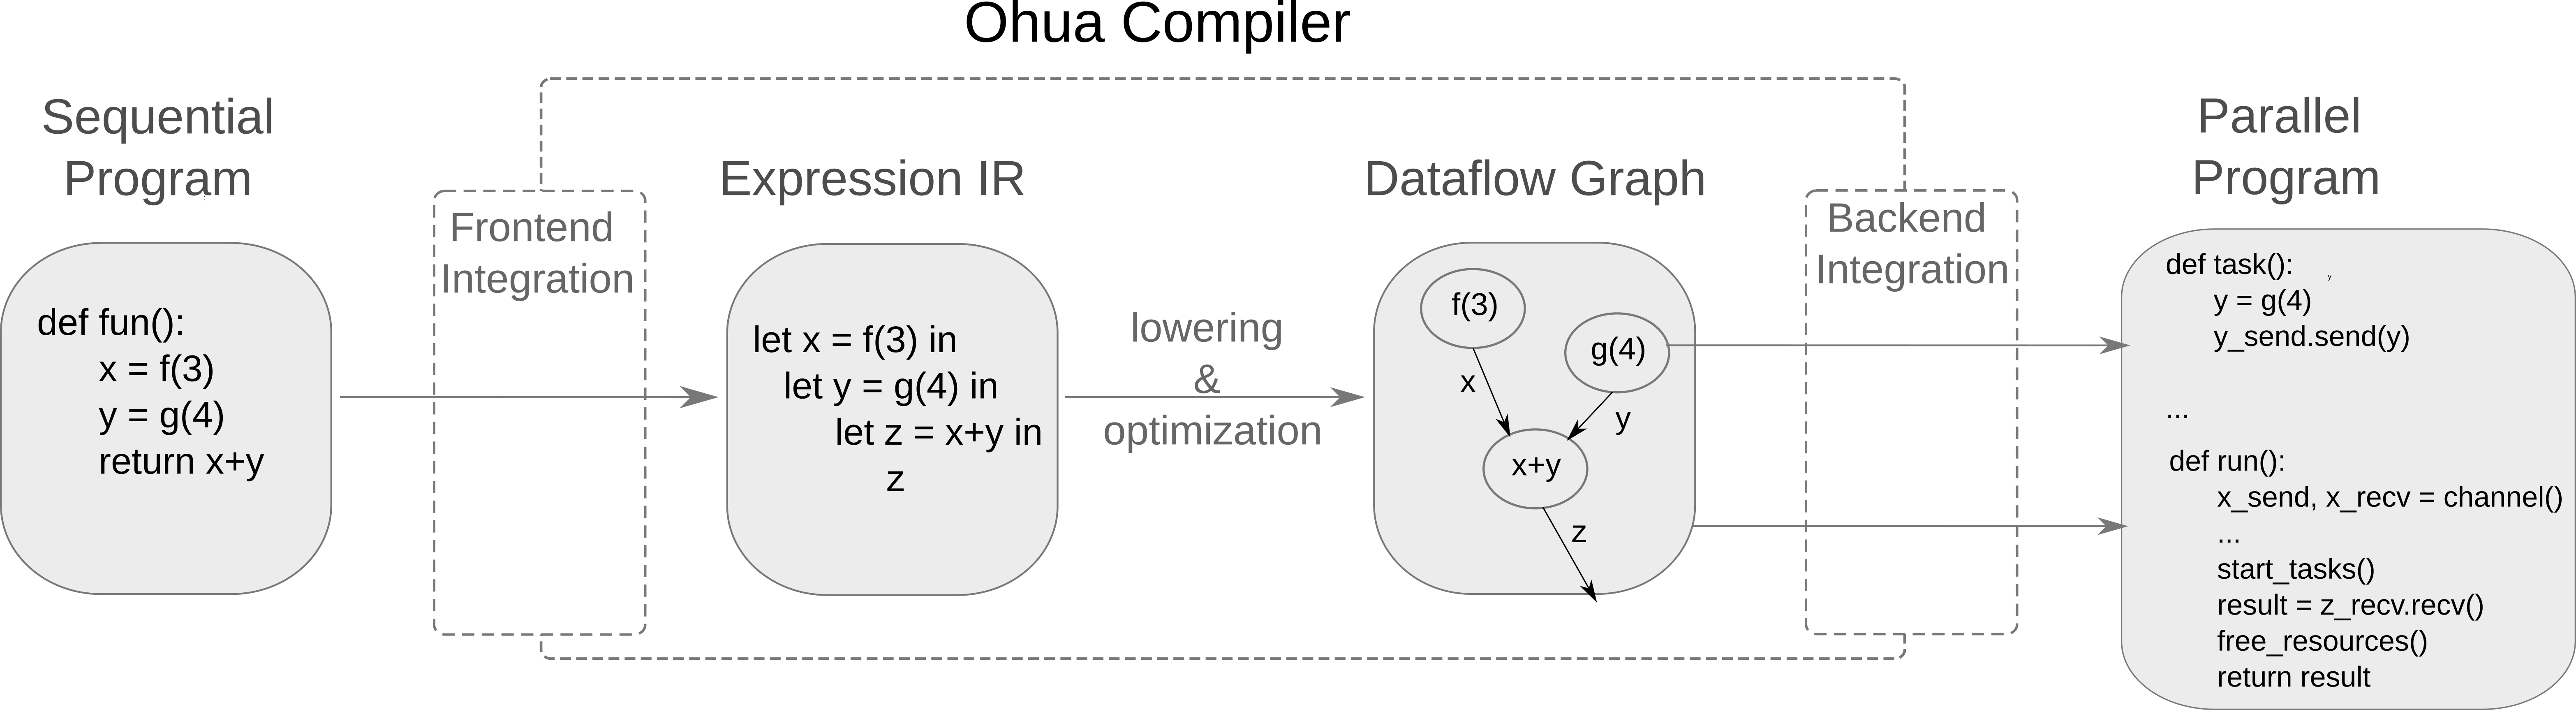
\includegraphics[scale= 0.36]{figures/ohua_fine_with_channels.png}
    \caption{Structural overview of Ohua and the code transformations}
    \label{fig:ohua_fine}
\end{figure}

In the \textbf{core compiler} itself there are two main representations of the code. One is Expression IR. This language is functional and based on the call-by-need lambda calculus. To transform input algorithms to this representation 
calls to other algorithms are inlined, renaming compiler passes ensure single static assignment form, and assignment expressions are refactored to applicative normal form. A simplified example of code before and after the transformation is shown in Listing~\ref{fig:funBodyTranslation}. A central conversion step in the compiler is the transformation of stateful calls to so called \emph{state threads}(\cite{wadler1992essence}, \cite{launchbury1994lazy},\cite{ertel2019stclang}). To generate race condition free tasks, Ohua forbids shared state use and only permits stateful computation inside methods. However, methods in an imperative language mutate objects in place and implicitly refer to the new, changed state by the same reference as before. The conversion of stateful calls to state threads makes the semantic of creating a new state upon calling methods explicit. In the code example in Fig.\ref{fig:funBodyTranslation}, the call \rust{someState.do()}, is internally transformed to explicitly take a state as an argument and return a new, mutated state. Thereby, function calls downstream to not need to access a shared memory to use stateful objects. Based on this explicit state threading, Ertel et al. \cite{ertel2019stclang, ertel2018supporting} developed functional representations for imperative control flow on stateful computations. For example, an imperative for-loop is translated to a so called \rust{smap} operation, which is essentially a fold operation of the loop body on the states manipulated inside the loop. \\

\begin{codefigure}
    \centering
    \begin{subcodefigure}[b]{0.45\textwidth}
         \centering
         \begin{minted}[fontsize=\small]{rust}
 fn algo(i){
   let someState = 
           other_algo(i);
   let a = someState.do()
   let b = f(a)
   return b
 }

 fn other_algo(i){
    let s = State::new(i)
    s
 }
            \end{minted}
         \caption{Input algorithm}
         \label{simplPyInput}
     \end{subcodefigure}
     \hfill
     \begin{subcodefigure}[b]{0.5\textwidth}
         \centering
         \begin{minted}[fontsize=\small, escapeinside=||,mathescape=true]{haskell}
let someState = 
        |$\lambda$| State::new (i) in
  let a, someState_0 = 
           |$\lambda$| do (someState, a) in
    let b = |$\lambda$| f (a) in
        b
        \end{minted}
        \vspace{15mm}
    \caption{Pseudocode of IR}
         \label{simplIR}
    \end{subcodefigure}
\caption{An algorithm is mapped to a nested let-expression with the innermost term representing its return value}
\label{fig:funBodyTranslation}
\end{codefigure}

The next representation in the compile flow is the Data Flow Graph (DFG) representation. Independent program tasks are encapsulated in the this representation and are explicitly assigned their incoming outgoing data channels. Besides function calls from the original program, this representation also contains control nodes that govern the data flow. For example if the input code contained a branching statement like \rust{if cond {f()} else {g()}} control nodes will be introduced to a) switch data flow between calls to \rust{f()} or \rust{g()} and b) to collect results from appropriate output channels of \rust{f()} or \rust{g()} depending on the condition. This representation also allows to merge certain nodes by fusing their code, as well as input and output channels. This is done for instance if a following node entirely depends on its predecessor and has so little work to do that it would hardly justify the overhead of spinning up an independent task in any backend implementation.\\

Which ultimately brings us to the \textbf{compiler backend} and backend integrations of Ohua. Backend integrations consist of two parts. The 'Language Backend' is only language specific. Similar to the frontend integration, it serves the purpose of translating code inside tasks from Ohua representation syntax back to the target language syntax. The 'Architecture Backend' is responsible for translating the 'nodes' and 'edges' of the DFG into a specific implementation for concurrent tasks, communication channels and a runtime for the graph. For example, there can be two different architectures for a given language: one implementing tasks as threads and one using processes, with both also generating appropriate channels and runtime code to execute the DFG. As we did not compile imported functions, the target language must match the input language, which is automatically ensured by the compiler. Architectures for the same language can be used interchangeably. This way Ohua can generate e.g. multi-threaded shared memory or fully distributed programs from the same input.\\

In the next section we will take a closer look at the restrictions and assumptions required to ensure that compilation works as expected.

\subsection{Programming Model}

The term programming model generally describes a relationship between syntax constructs in a programming language and their concrete semantics in a particular execution environment. In the case of Ohua, the programming model includes, on the one hand, the supported input syntax and the assumptions made about the supported terms of the input language. On the other hand, it specifies how these terms are translated into a dataflow graph and what assumptions Ohua makes about the implementation of nodes, edges, and runtime of the DFG. First we will look into the supported input syntax and assumed semantics. 

\subsubsection{Input Syntax and Semantics}
We already know that Ohua's basic input units are algorithms, i.e. pure functions inside the compile scope. Table~\ref{tab:FrontendIR} depicts the language definition of the frontend representation described before. Any syntax construct of the input language has to be mapped to the according terms of this language to be compiled. In the following paragraphs we will describe the accepted syntax constructs and the semantics the programming model expects them to have. \\


\begin{table}[ht]
\resizebox{\columnwidth}{!}{%
    \begin{tabular}{l c l l}
        \multicolumn{4}{l}{\emph{Patterns:}}\\
        $p$ & $::=$ & $x\ |\ (x,~\ldots ,~x)\ |\ ()$ & named variables, tuples or unit\\
        \multicolumn{4}{l}{\emph{Expressions:}}\\
        $e$ & $::=$ & $e$ & named expression in host language\\
        & $|$ & $\textbf{1},\textbf{2},\textbf{3}, \ldots \ |\ \textbf{true}\ |\ \textbf{false}\ |\ \textbf{()} $ & typed literal in host language\\
        & $|$ & $\textbf{let}\ p\ \textbf{=}\ e\ \textbf{in}\  e$ & lexical scoping \\
        & $|$ & $e\ e$ & application\\
        & $|$ & $\boldsymbol{\lambda} [p,~\ldots ,~p]\textbf{.}\  e$ & abstraction \\
        & $|$ & $\textbf{if}\ e\ \textbf{then}\ e\ \textbf{else}\ e$ & conditionals\\
        & $|$ & $\textbf{map}\ e\ e$ & map first expression to second\\
        & $|$ & $\textbf{bind}\ e\ e$ & bind an expression representing a state to  \\
        & & & an expression representing a function to act on this state \\
        & $|$ & $\textbf{stmt}\ e\ e$ & expression whose return value is ignored\\
        & $|$ & $\textbf{seq}\ e\ e$ & \\
        & $|$ & $\textbf{(}\ e\ \textbf{)}$ & tuple of expressions \\
    \end{tabular}%
    }
    \caption{Definition of the Expression IR}
    \label{tab:FrontendIR}
\end{table}

\textbf{Function Calls:} Beside algorithms, Ohua supports stateful and stateless function calls, i.e. methods and pure functions, imported into the scope. Pure functions are expected to be side effect free. In particular, the programming model assumes that pure functions do not implicitly manipulate their arguments. This excludes, for instance, functions that manipulate their arguments by reference. If the output of a pure function call is not used, it is considered to have no effect and is removed during compilation. 

Stateful function calls, on the other hand, are expected to manipulate the object they are called on, i.e. have a side effect. Consequently, they are not removed regardless if the output is used. 
Any stateful computation is expected to happen exclusively and explicitly using method calls and also method calls are expected to only manipulate the object state itself. This also entails the requirement that the state is not 'leaked' via return values. For example, in the method call \rust{let x = SomeState.do_stuff();}, \rust{x} must not be, or contain, a reference to \rust{SomeState}. We already assumed that other functions do not manipulate \rust{SomeState} when using \rust{x} as argument. However, without this 'leaking assumption' it would be possible to call \rust{x} as a stateful object, thereby implicitly manipulating the state of \rust{SomeState}. This implicit semantic is not handled currently and would be lost in the distributed output code. 

Functions need to be typed or type-able by the frontend integration. To correctly annotate the types in generated code, at least to the extent required for any particular backend and architecture, Ohua needs to extract type information from the input code. Specifically the argument types of each function call are extracted and preserved in the different IRs as typed function literals capturing the argument types of each function call. \\

\textbf{Loops}: Ohua supports bound and unbound \rust{for}-loops. They are transformed into parallelizable pipelining of the independent calculation steps inside the loop. Inside for-loops, each state from outside the loop must be used at most once to enable the accumulation of state changes in a single node for each object. Conditional loops (\rust{while} or \rust{do-while}) are as of the beginning of this work not supported, but can be expressed using recursion.\\

\textbf{Recursion}: Ohua supports recursion with some notable restrictions. Recursive algorithms must be tail recursive, the recursive call must be located in the if-branch, and the return value must be in the else-branch of recursion. Furthermore, either one must be the only statement in each branch respectively. As return values only single variables are supported. Recursive loops will not yield any pipelining or parallelization but a loop executed for one input at a time. This is due to the semantic of recursion, being a repeated function on a state, where the result of each step depends not only on that step but also on previous results.
Currently, the output of recursive algorithms cannot be used in an assignment, i.e. a recursive call can only be the last statement in another algorithm and return the calling algorithm's final result. \\

\textbf{Branching:} Branching is supported in case of simple if-else expressions, where both branches must be present. Also, if-else statements, as for instance present in the Python syntax, are currently not supported. This is because those statements have a different execution semantic than expressions, i.e. branches that do not return a value but have side effects on variables from the surrounding scope, so they need to be implemented separately. In addition, it is currently not possible to use stateful functions in branches.\\

\textbf{Return, Continue, Break:} Ohua currently does not support any forms of early return of conditional execution except for recursion and branching as described before. Therefore, \rust{break} and \rust{continue} are generally not supported at the moment, while \rust{return} is supported only for Python and only at as the last statement of a function block, because contrary to Rust there is no implicit value return in Python. \\

\textbf{Variables and Literals:} There are two categories of variables. Local variables are bound inside algorithms, environment variables are bound in outer scope. Thus, environment variables are basically arguments of the algorithms, but can also be imported or globally defined names. Ohua supports mutable and immutable local variable bindings. Local variables can either be used as a state, or as an argument to a function call. If it is used as an argument it can only be used once, if it is used as a state, it may be used more than once except, as explained before, inside loops. Environment variables cannot be used as a state directly\footnote{This changed during the course of this work. Now arguments to algorithms can be used directly as a generator for a for-loop.}, but can be used several times as function call argument. The underlying assumption of this distinction is that environment variables will be available in scope for all nodes created from an algorithm, while locally bound variables are sent to the consuming node. This assumption becomes relevant in architectures where the generated tasks have no access to a common global scope. In those cases, environment variables are not available to the task via a closure mechanism. This will be the case for \md tasks. Finally there is a limited set of literals that is directly supported in the input. This includes integers, booleans, strings and unit literals. Other literals must be wrapped in a function call currently (simple binary operations are sufficient here e.g. to compile \rust{let x = 17} one could write \rust{let x = 17 + 0}).\\

Many of the current limitations are only due to lack of implementation. For example, there is no formal reason to allow recursive calls only in the if branch. These limitations will be fixed in the future. At the moment, however, they are the main reason why control flow expressions cannot be freely combined. That is, there are currently restrictions on the frontend language that are not reflected in the language itself.


\subsubsection{Enforcement}

Conformity with the allowed syntax subset is automatically implemented by each language integration, as it has to translate the input syntax to the frontend language. However, this is only a syntactical conversion. Except for tracking the annotated type of named variables, the compiler does no further semantic analysis of the input code. This means that to comply with a programming model requirement it is sufficient to match the expected syntax, but not necessarily the expected semantics. Take for example the requirement to use each variable only once as a function input. To use a variable \rust{x} twice, a programmer needs to return it twice from a function call \rust{let (x1, x2) = fun()}. However, she can freely decide whether \rust{x1} and \rust{x2} are copies or only references of \rust{x}, matching the expected syntax but not the expected semantics of the programming model. The result might still be valid output, but it is the responsibility of the programmer to ensure validity of reference passing in the concurrent output. Likewise, the use of global mutable state can be encapsulated in function calls. \\

In general, enforcement of the programming model is currently not separately implemented and in some case lacking completely. Violations of the programming model will either lead to runtime errors during any point of compilation or may lead to invalid output code. The latter case was not an obvious problem in Rust, as Rust itself enforces borrowing rules and therefore a considerable part of Ohua's limitations. However, this is not generally the case in other languages, so tests were added in the course of this work to ensure compilation failure upon violations of the programming model.


\subsubsection{Backend Language and Process Abstractions}
\label{subsec:BackendRequirements}
The terms of Ohua's backend language are depicted in Table~\ref{tab:DFGdef}. As complex syntax constructs of the input language are removed in the frontend, most of the terms in the backend language are basic constructs of any imperative language, as variables, literals, assignments, and simple control flow terms. To generate the code for Ohua-introduced control nodes, some \emph{specific functions} are also required to be present in the host language. In particular, the control of loop execution requires implementations for list handling, as well as the functionality for \emph{iterable objects} of the host language, to test if they have a fixed size and if so retrieve this size information. \\

Obviously, the backend language also entails the notion of named and typed channels, their sending and receiving ends, and sending and receiving of variables a means of communication among the tasks of the data flow graph. 

\begin{table}[ht]
\resizebox{\columnwidth}{!}{%
    \begin{tabular}{l c l l}
        \multicolumn{4}{l}{\emph{Typed Task Expressions:}}\\
        $e$ & $::=$ & $ x\ | \textbf{1}, \ldots \ |\ \textbf{true}\ |\ () $ & variables, simple literals \\
         & $|$& $ \textbf{funRef}\ | ref \textbf{envRef}\ !HostExpr  $ & function and environment references \\
        & $|$ & $ x (e,~\ldots,~e) |\ Obj.x (e,~\ldots,~e)  $ & pure function and method calls\\
        & $|$ & $\textbf{let} x\ \textbf{=}\ e\ \textbf{in}\ e |\ \textbf{=}\ e$ & scoped bindings and assignments \\
        & $|$ & $\textbf{stmt}\ e\ e$ & statement \\
        & $|$ & $x\textbf{\_receiver.receive()} $ & expression to  receive data \\
        & $|$ & $x\textbf{\_sender.send(}x\textbf{)} $ & expression to send data \\
        &\multicolumn{3}{l}{--control flow--}\\
        & $|$ & $\textbf{while True:}\ e$ & \\
        & $|$ & $\textbf{for}\ x\ \textbf{in}\ x\ \textbf{do}\ e$ & \\
        & $|$ & $\textbf{repeat}\ (x\ |\ l)\ e$ & \\
        & $|$ & $\textbf{while}\ e\ e$ & \\
        & $|$ & $\textbf{if}\ e\ \textbf{then}\ e\ \textbf{else}\ e$ & \\
        &\multicolumn{3}{l}{-- specific functions, required for control nodes --}\\
        & $|$ & $\textbf{newList}\ $ & create a list \\
        & $|$ & $\textbf{append}\ x\ e $ & append t to x \\
        & $|$ & $\textbf{hasSize}\ x$ & $[a]$ \means Bool \\
        & $|$ & $\textbf{size}\ x$ & $[a]$ \means Int \\
        & $|$ & $\textbf{(}\ l,\ l\textbf{)}\ | \  \textbf{(}\ x,\ x\textbf{)}$ & Tuple of literals or bindings\\
        & $|$ & $(x ,\  \_ )$ & First\\
        & $|$ & $(\_ ,\ x )$ & Second \\
        & $|$ & $ x++$ & Increment \\
        & $|$ & $ x--$ & Decrement \\
        & $|$ & $ \textbf{not}\ e$ & \\
        \multicolumn{4}{l}{\emph{Communication Channels:}}\\
        $channel\ $& $::$ &$\textbf{channel}\ x$& Typed channel, i.e. incoming and outgoing end for variable x\\
        & $|$ &$x\textbf{\_receiver}$& Typed receiving end of a  channel  \\
        & $|$ &$x\textbf{\_sender}$ &Typed sending end of a channel  \\
    \end{tabular}%
    }
    \caption{The terms of Ohuas backend language used to represent the DFG. Language specific backend integrations translate this language to generate the output program.}
    \label{tab:DFGdef}
\end{table}

A major advantage of compiling with Ohua is that the generated dataflow-based language is deterministic. That is, a correct, deterministic, sequential program becomes a correct, deterministic, concurrent program by compilation. Formal verification of the compiler transformations to proof this claim and formalize the programming model is currently an ongoing task. Nevertheless, we can already clearly describe the assumptions concerning the concrete implementations of nodes, edges and the runtime each architecture must provide.\\

Specifically, we assume for the implementation of nodes and runtime that:
\begin{enumerate}
    \item Nodes do not share mutable memory. However, the architecture provides access to environment references, which may be global constants, imports, and (most importantly) the arguments of the compiled algorithm.
    \item There can be more nodes than the runtime is capable of running concurrently and there is no explicit scheduling. Therefore we assume cooperative multitasking, i.e. nodes waiting for input will free computation resources for other nodes.
    \item The runtime instantiating the nodes is capable of ending them and freeing resources.
\end{enumerate}

Since it is a data flow language, the execution of the programs is controlled by the data flow. This results in the following assumptions for the implementation of the edges: 

\begin{itemize}
    \item[i)] all data are transferred in order,
    \item[ii)] there is no implicit use of default arguments (default arguments are in general possible, but there has to be an explicit signal for every computation in a node and every parameter it uses that this parameter is 'None' and should be replaced by the default value for this particular execution round/loop),
    \item[iii)] receiving is blocking (this closely relates to ii) in the sense that there must not be a calculation or result passed on while it is not clear whether a term of that calculation just has not arrived at the moment of calculation),
    \item[iv)] all types visible in the compile scope are sendable in the given architecture.
\end{itemize}

Contrary to the assumptions on the input code, the assumptions about the architecture and backend integration cannot be validated inside the compiler. 
    
\section{Micro- and Unikernels}

General-purpose operating system have to provide a broad range of functionalities to connect application layer to hardware layer. This includes user interfaces (graphics), networking, security, device drivers, and most obviously the functionality required for program execution and memory management, which may also include virtualization mechanisms for programming languages as Java and Python. To enable efficient execution and communication between the components, Unix-like operating systems, for example, are often implemented as monolithic kernels. In monolithic kernels the system services (daemons) and drivers have direct access to the hardware and the shared memory. \\

However, this approach has considerable downsides. Since drivers and daemons run in kernel mode, they have full rights and access to the resources of all other processes. This means that in the event of a vulnerability in one of the components, the entire system is affected in principle. In particular third-party device drivers were notoriously faulty and a portal for exploits\footnote{Recent example of \href{https://nakedsecurity.sophos.com/2021/03/17/serious-security-the-linux-kernel-bugs-that-surfaced-after-15-years/}{driver bugs} in the Linux kernel }. Also, many applications do not require most of the services provided by those general purpose systems. For example, a microservice that merely answers simple requests to a key-value store only needs the functionality of the network stack and the file system. Libraries and system functions for additional user or device interfaces only unnecessarily increase the complexity, memory consumption and attack surface of the service. \\

Two alternative concepts of kernels are micro- and unikernels. Figure~\ref{fig:kernels} shows how user applications, drivers and system services, and the hardware layer are compartmentalized in each of these kernel architectures in principle. Basically, the idea of microkernels is to reduce the code run in kernel mode to the absolute minimum required to access the actual hardware layer, while unikernels are often based on a microkernel, but also give non-essential components required for a specific app to run direct access to hardware resources. We will briefly introduce the two concepts, as well as the related concept of library operating systems here.

\begin{figure}[H]
    \centering
    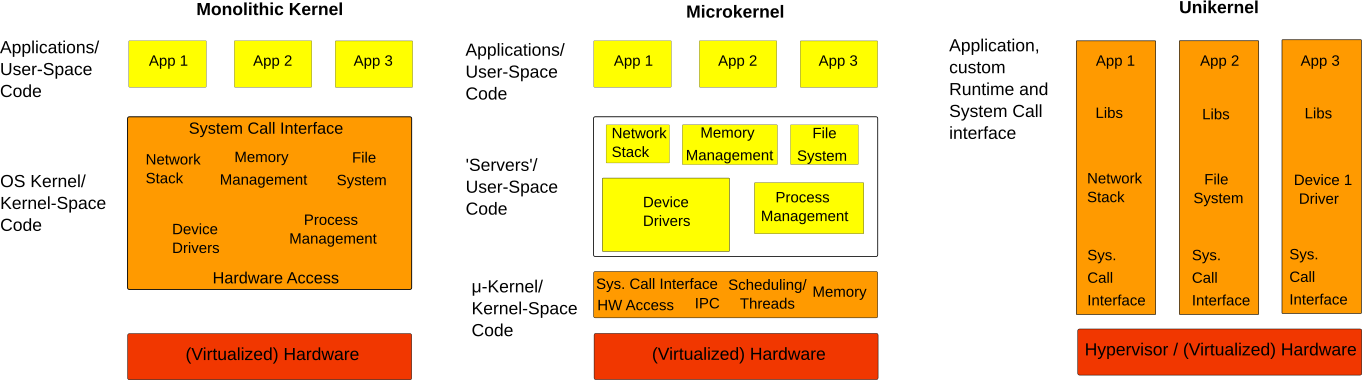
\includegraphics[scale= 0.36]{figures/kernels.png}
    \caption{Structural comparison of Monolithic, Micro- and Unikernels }
    \label{fig:kernels}
\end{figure}

\textbf{Microkernels$\blacktriangleright$} Microkernels follow a \textit{minimality principle} formulated by Liedtke~\cite{jochen1995mu} as \\

\emph{''More precisely, a concept is tolerated inside the $\mu$-kernel only if moving it outside the kernel, i.e. permitting competing implementations, would prevent the implementation of the system's required functionality.''}\\

The central motivation for microkernels is the reduction of privileged, low-level code executing in kernel mode. Based on the insight that large code bases of monolithic kernels come at the cost of a large potential for bugs in privileged, low-level (and therefore hard to check) code, concepts to minimize kernels (and therefore attack surface) date back to the 70$^th$ \cite{hansen1970nucleus}. Concepts like the Mach kernel \cite{accetta1986mach}, separation kernels\cite{rushby1981design}, or isolation kernels \cite{whitaker2002scale} where developed to minimize and isolate kernel space code, to increase security, and enable verification.  \\

The minimality principle basically limits the essential components of kernel-to-memory management (i.e. providing access and access control to address spaces), CPU allocation (i.e. providing access to the CPU in any form of process or thread abstraction and scheduling), and inter-process communication (IPC). Other services, such as I/O, device drivers, networking, and others are run as userland processes, although there might be further distinctions from actual user processes. In addition to the advantage of the smaller attack surface, the low memory requirement also makes microkernels advantageous, especially for embedded systems. \\

This design comes with an inherent performance penalty. In a monolithic system a userspace application requiring access to hardware or system services would cause a single context switch to kernel mode. The request would be answered and the result returned to the userspace process. In a microkernel, however, the request of the user application will be forwarded by the kernel via IPC, e.g. to a driver process that again answers via IPC indirected through the kernel. In this simple scenario, the number of context switches doubles from two to four. Also, the communication among system services is just function calls in monoliths, while it again involves IPC and four context switches for each invocation among services. \\

Currently existing examples of microkernels are L4 (formerly L3 \cite{liedtke1993persistent}), Minix \cite{herder2006minix}, Singularity \cite{hunt2005overview} or the QNX microkernel OS\cite{hildebrand1992architectural} used in embedded systems for example in phones, or as real time OSs in cars.\\

\textbf{Unikernels\cite{madhavapeddy2014unikernels} $\blacktriangleright$}: Unikernels also tackle the problem of large code base and attack surface in monolithic kernels. However, they follow a different approach concerning process isolation. The 'uni' in unikernels refers to the idea of compiling a specific kernel for each application or even component of larger applications. Basis for compilation is a library operating system written in rather high level languages, the user program, and a configuration file to specify the target architecture and the required library components. Library operating systems provide functionalities of monolithic kernels as independent library implementations. For example, device drivers for physical NICs are implemented in libraries that can be combined with potentially different implementations of the TCP/IP stack. Examples of library operating systems are  MirageOS\cite{madhavapeddy2013unikernels}, Graphene~\cite{tsai2014Graphene}, IncludeOS~\cite{bratterud2015includeos} or Unikraft~\cite{kuenzer2021unikraft}.
In the compiled unikernel, all processes run with kernel privileges and have direct access to the hardware or hardware abstraction layer (e.g. a hypervisor). This reduces size and attack surface compared to monolithic kernels and has, unlike monolithic and microkernels, no IPC overhead for context switches. 
It is not well suited and not intended to be used for multi-user scenarios. However, large applications can be realized with unikernels by distributing the app components into several distinct unikernels. In cloud applications, this setup allows the hypervisor to scale only required parts of the application. Examples of this principle are CubicleOS~\cite{sartakov2021cubicleos} and FlexOS~\cite{lefeuvre2021flexos}.

\section{The M\textsuperscript{3} Operating System}
\subsection{The Concept}
M$^3$\cite{Asmussen:M3x} is a microkernel concept/architecture for distributed and potentially heterogeneous architecture, as for example different embedded processors cooperating in modern cars. It comprises a hardware and a corresponding software, i.e. OS and kernel design. Specifically, the hardware design describes the components necessary to connect and control separate chips, e.g. for broadband communication, signal processing (camera, GPS), or cryptographic operations, while the corresponding operating system provides communication and access to the hardware for the apps running on each component.\\

An overview of the design of M$^3$ is shown in Figure~\ref{fig:m3}. The architecture is composed of tiles, communicating with each other via data transfer units (DTU). There is only one tile that runs the actual microkernel. This tile is also the only one requiring a general purpose core (GPC) as underlying hardware. The computing units (CU) inside the other tiles might be general purpose CPUs, FPGAs, DSPs or fixed-function accelerators. Processes on CUs run independently and isolated from each other. They can however communicate to each other via the DTUs. The kernel is responsible for scheduling tasks on the CUs. Running tasks are called activities. On tiles using CPUs, an activity is basically a running system thread. Via the DTUs, the kernel can also control context switches between activities on the CUs and establish communication relations between activities. By default, activities run in their own address space and are disconnected from each other. To establish a connection, an activity \code{A} would once request the kernel to connect, for instance to an activity \code{B} running the network stack. Once that connection is established, the activities can directly communicate without involving the kernel again, which eliminates some of the communication overhead in other microkernel systems. 

\begin{figure}[H]
    \centering
    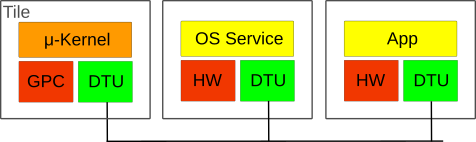
\includegraphics[scale= 0.7]{figures/m3.png}
    \caption{The m3 architecture is composed of tiles, communicating via data transfer units (DTUs).}
    \label{fig:m3}
\end{figure}

In Section~\ref{subsec:BackendRequirements} we discussed the assumptions Ohua makes about the backend architectures' tasks and channels. In particular, we noticed that tasks have to be cooperatively scheduled and channels have to ensure in-order, guaranteed delivery. Here we take a look if these requirements are fulfilled by M$^3$.\\

When activities are idle, they notify the kernel, which can then schedule another activity. So cooperative scheduling is given. Communication channels are unidirectional, first-in-first-out connections. Activities are not aware if their communication partner is currently running or suspended i.e. if the context was switched by the kernel. The hardware (i.e. the DTU of the receiving tile) detects attempts to communicate with a not-running activity and errors back to the sending activity. Upon such error, the sending activity invokes the kernel to schedule the required receiving activity. The kernel buffers messages for the receiver in this case. Despite this fallback mechanism, the authors state that message delivery has only-once semantic, so data access can/must be repeated if necessary upon failure. 

\subsection{The Rust API}
\md provides a Rust integration to access its abstractions of processes and channels. Here we briefly describe the main features of this API. A simple example of how an activity can be instantiated is shown in Listing~\ref{fig:startingActivity}\footnote{Example adapted from \href{https://github.com/Barkhausen-Institut/M3/blob/master/src/apps/rustunittests/src/tactivity.rs}{\md Rust unit tests}}. Activities can be initiated either on a common tile or on several tiles. In the example, the tile of the parent process is used. The API uses a closure syntax to define activities. However, those definitions have no closure semantic, i.e. they do not enclose definitions from the surrounding scope.\\

To pass capabilities and file descriptors to a child activity, the attribute \rust{activity.data_sink()} can be used to serialize data into the process memory. This data can be accessed from inside the activity code using \rust{data_source()}. Serialization is implemented in a custom \rust{Serializer} based on the \rust{serde} crate. We need this mechanism, as shown in the example, to pass send and receive gates to the activities. For simple environmental variables, the API provides a separate mechanism using \rust{m3::env}. This basically provides a global key-value store in which variables can be stored before the definition of an activity, retrieved by key inside the activity, and deleted after the activity definition to not pollute the namespace.\\


\begin{codefigure}[ht]
    \centering
    \begin{minted}[fontsize=\footnotesize]{rust}
fn run_send_receive(t: &mut dyn WvTester) {
    // Get a descriptor of the current tile
    let tile = Tile::get("clone|own");
    // Initialize a new activity on the current tile
    let mut activity = ChildActivity::new_with(tile, ActivityArgs::new("test"));

    // initialize send and receive gate with message order, size and credits 
    let rgate = RecvGate::new(math::next_log2(256), math::next_log2(256));
    let sgate = SendGate::new_with(SGateArgs::new(&rgate).credits(1));

    // make receive gate avaible in the activities namespace
    activity.delegate_obj(rgate.sel());
    let mut dst = activity.data_sink();
    dst.push(rgate.sel();

    // define activity 
    let activity = activity.run(|| {
        ...
        // make receive gate available inside activity
        let mut src = Activity::own().data_source();
        let rg_sel: Selector = src.pop().unwrap();
        let rgate = RecvGate::new_bind(rg_sel);

        // receive 
        let mut res = recv_msg(&rgate));
        let i1 = res.pop::<u32>();
        let i2 = res.pop::<u32>();
    });

    send_vmsg!(&sgate, RecvGate::def(), 42, 23));
}
    
    \end{minted}
    \caption{Example of creating and running a Rust activity on \md}
    \label{fig:startingActivity}
\end{codefigure}

Concerning process communication, the API provides different mechanisms (mainly depending on the size of the data to be transmitted) of which direct sending over channels is the most relevant to us. \md manages communication among processes using capabilities. The capability to directly send to or receive from another process is implemented as \rust{Gate}s in the \md Rust API. Gates are synchronous, directed one-to-one connections, so there are send gates \rust{SGate} and receive gates \rust{RGate}. Receive gates are instantiated with a maximum message size and a maximum overall size of the message buffer to prevent memory overflows in limited environments. The absolute (system immanent) maximum message size is 2 kb. Send gates are instantiated with a number of credits. With each message send, one credit is used. The receiver can return those credits by answering on a received message. Note that this mechanism is hidden inside the \rust{recv_msg} and \rust{send_vmsg!} calls. Both are or contain macro calls to generate and receive responses upon message receipt to pass back sending credits. \\

Apart from the credit system, sending messages is straight forward, as known from most pipe-like interfaces. Receiving is done in two steps. First a receive stream is requested using \\
\rust{let stream = rgate.recv_msg()}. This is a blocking call, that will return upon available messages arriving at the gate. The second step is calling \rust{let msg = stream.pop()}, which is non blocking. This call can be done arbitrarily often on an existing stream but will fail if there are no more messages in the stream. Finally, a limitation of the current \md API is that the standard library is not supported. There is a separate implementation of \rust{std} with essential functions but partly different function signatures. For smoltcp itself this limitation is not relevant, since it is written without using the standard library. In contrast, the libc API is a necessary part of smoltcp and is supported by \md. 

\subsection{Existing \md Architecture Integration}
Ohua already features an architecture integration for Rust on \md. It is built on a simplified API of \md that provides two main encapsulations, the \rust{channel()} call and the \rust{activity!} macro. Listing~\ref{fig:OhuaM3Wrapper} shows how an activity can be created using those functionalities. The function \rust{channel} basically wraps the initialization of pairs of send and receive gates with default message orderings, a default message size, and a default of one send credit. This allows to create channels basically the same way as in pure Rust or Python. The \rust{activity!} generates code to 1) instantiate a \rust{ChildActivity} on the current tile, 2) delegate the given gates to the activity, and 3) bind and activate the gates inside the activity. This again basically resembles the initialization of a thread in pure Rust. 


\begin{codefigure}[ht]
    \centering
    \begin{minted}[fontsize=\footnotesize]{rust}
    use funs::hello_world;
    
    fn test() -> String {
       use m3::com::channel::{Sender, Receiver};
       use m3::activity;
       let (a_0_0_tx, mut a_0_0_rx) = channel(); 
        activity!(
            (|a_0_0_child_tx: Sender| {    
                let a_0_0 = hello_world();
                a_0_0_child_tx.send(a_0_0)?;
                Ok(())
              }
            )(a_0_0_tx)
        );
        a_0_0_rx.activate()?;
        a_0_0_rx.recv::<String>().expect("Error message")
    }

    \end{minted}
    \caption{Example of creating an activity using the simplified \md Rust API}
    \label{fig:OhuaM3Wrapper}
\end{codefigure}

However, as previously explained, activities in \md are not closures. This means that in order to use environment variables, an additional mechanism will be necessary. This is currently not part of the architecture integration.

\section{smolTCP}
smolTCP~\cite{smolTCP} is a Rust-based open-source library for network stack implementations. It runs entirely as a user space application. It also provides conditional compilation features to build applications without heap allocation. This makes smoltcp and applications built with it amenable to be used in microkernels such as M$^3$\cite{Asmussen:M3v} and embedded systems such as ARTIQ (e.g. \cite{lam2021combining}). In fact, the microkernel operating system Redox\cite{redoxwebsite}, as well as \md itself, already use smoltcp for their network stack implementation. So in both systems, smoltcp is used to create a network stack as a sequential, userspace service. This means that, in contrast to the application to be developed in this thesis -- the TCP/IP layer, the actual network layer or system interface and the user application communicate with each other via shared memory. \\

The design of the library is structured according to typical TCP/IP layering. We will briefly introduce the three main layers or components, respectively, that are relevant in this work\footnote{For more information see the documentation at \url{https://docs.rs/smoltcp/latest/smoltcp/}.}.


The \rust{socket} module provides different socket abstractions implementing the TCP, UDP, IGMP or DHCP protocols, respectively, as well as for raw sockets. Common features of all those abstractions are keeping track of inbound and outbound data in socket buffers and implementing functionality to package or unpack those data according to the implemented protocol. The sockets keep also track of additional state information, relevant for their respective protocol e.g. TCP or DHCP client states, hop limits, window sizes, etc.\\

The \rust{iface} module provides the abstractions of the IP layer. The most important structure is \rust{Interface}. In an inner component of the interface (\rust{InterfaceInner}), the state data of the IP layer are stored. This includes the IP address of the interface, a routing table, a neighbor cache, and the hardware address (depending on the transport medium according to Ethernet or IEEE 802.15.4 standard). Accordingly, the generation and interpretation of IP headers for outgoing and incoming packets are also tasks of the 
\rust{InterfaceInner}. In the currently official variant of smoltcp, the Interface also contains a field \rust{Device}, holding an abstraction of the physical network layer, and a \rust{SocketSet} to manage all sockets belonging to the interface. Smoltcp is under ongoing development and so, in the recent implementation state, \rust{Device} and \rust{Sockets} are no longer part of the interface, but independent structures passed to it to process packets from sockets to device and vice-versa. We will discuss the implication of this in further detail in the Section~\ref{sec:ImplSmoltcp}. \\

Finally, the physical layer is implemented in the \rust{phy} module. It provides different implementations of the \rust{Device} trait, to connect the application to the underlying operating systems loopback or tuntap interface or raw sockets. Implementors of the \rust{Device} trait provide the methods \rust{receive}, \rust{transmit} and \rust{capabilities}.\\

The actual transfer of packets from the interface to the device is realized via sending and receiving tokens. We explain this in a little more detail here, because it exemplifies a characteristic of the smoltcp code. A successful call to \rust{device.receive()} will yield a tuple of a receive token \rust{RxToken} and a send token \rust{TxToken}. The former will contain the actual received content as a private field, the latter contains a reference to the device specific storage for outgoing packets. In case of tuntap and rawsocket devices, this reference is a file pointer provided by the operating system. In Lising~\ref{fig:TokensAndClosures} the a slightly simplified implementation of a sending \rust{TxToken} for raw sockets and the usage of such token to send an Ethernet frame are shown. Two things become apparent. First, the memory for the packets is allocated only at device level upon consuming a token. Second, any structs needed to construct the frame are instantiated in a closure passed as an argument to \rust{tx_token.consume()}. As closures are realized via fixed size structs on the stack frame of the called function, this technique enables smoltcp to work without heap allocation and is used heavily in the code. This principle is used in a cascading manner i.e. \rust{dispatch_ethernet} itself also receives a closure capturing objects from the calling scope.\\

Obviously, one implication of separating the layers of smoltcp to different, memory separated components is that this kind of memory efficiency cannot be maintained. 

\begin{codefigure}[ht]
\centering
\tabskip=0pt
\valign{#\cr
    \hbox{%
    \begin{subcodefigure}{.41\textwidth}
    \centering
     \begin{minted}[fontsize=\tiny]{rust}
// Sending Token for RawSocket
pub struct TxToken {
    lower: Rc<RefCell<sys::RawSocketDesc>>,
}

impl phy::TxToken for TxToken {
    fn consume<R, F>(
    self, 
    ..., 
    f: F) -> Result<R>
    where
        F: FnOnce(&mut [u8]) -> Result<R>,
    {
        let mut lower = self.lower.borrow_mut();
        let mut buffer = vec![0; len];
        let result = f(&mut buffer);
        match lower.send(&buffer[..]) {
            Ok(_) => result,
            // Error handling 
        }
    }
}
     \end{minted}
    \end{subcodefigure}%
  }
  \cr
  \noalign{\hfill}
    \hbox{%
    \begin{subcodefigure}{.57\textwidth}
    \centering
    \begin{minted}[fontsize=\tiny]{rust}
        //Interface using a TxToken to send a frame
        pub fn dispatch_ethernet<Tx, F>(
        &mut self, 
        tx_token: Tx, 
        buffer_len: usize, 
        f: F) -> Result<()>
        where
            Tx: TxToken,
            F: FnOnce(EthernetFrame<&mut [u8]>),
        {
            let tx_len = EthernetFrame::buffer_len(buffer_len);
            tx_token.consume(self.now, tx_len, |tx_buffer| {
                ...
                let mut frame = EthernetFrame::new(tx_buffer);
                let src_addr = {...};
                
                // closure from outer scope:
                f(frame);
                Ok(())
            })
        }
    \end{minted}
    \end{subcodefigure}%
  }
  \vfill
  \cr
}
\caption{Sending and receiving packages is implemented via Tokens exposing a \rust{consume} method, taking closures as argument that process the send or received content. This way, memory allocation can be constrained a) to the device layer and b) to the stack if necessary.}
\label{fig:TokensAndClosures}
\end{codefigure}

\section{Rust}
\label{subsec:Rust}
The main questions of this thesis are i) What requirements must a sequential program meet in order to be converted into a concurrent program in a semantics-preserving way? and ii) What steps are necessary for the conversion? Rust as a programming language is particularly well suited to investigate these questions. This is due to Rust's extended type system that cannot only enforce well-typedness of a program but also statically ensure the validity of references and therefor safety of memory usage at runtime. The two central concepts enabling this are \emph{ownership} and \emph{lifetimes}. \emph{Ownership} is used to ensure memory safety in (safe) Rust. In particular, it allows the Rust compiler to ensure at compile time that no two pieces of code can modify an object at any time, i.e. that at runtime there is never more than one reference to an object that allows write access. \emph{Lifetimes} extend the concept of ownership to track the validity of references. This model does not only prevent frequent errors in sequential programs, it also enforces already a substantial part of the assumptions of a distributed programming model. Therefore, necessary restrictions of a distributed, concurrent programming model are particularly well to be examined in Rust, because they are already enforced in the sequential code. In Chapter~\ref{Chapter:Implementation}, we will refer to those concepts and their implications for our findings. So to better understand these implications, we will first take a closer look at the rules of ownership and lifetimes here.\\

\textbf{Ownership:} Rust has neither garbage collection nor does the user need to free and allocate memory herself. Instead, Rust's runtime manages memory using ownership and lifetime rules. The Rust compiler ensures, for most types statically, that there is exactly one \emph{owner} of each value, i.e. one variable holding it, created either on heap or stack. When this owner goes out of scope (i.e. when the scope it has been declared in ends), the value is cleared from memory without the need for extensive reference tracking garbage collection.
This is realized by automatic implementations of the \rust{drop} function for every type. A call to \rust{drop} is added automatically by the compiler for each variable as it goes out of scope.\\

Ownership has a different implementation for values located on the stack and on the heap. For values stored on the stack, the owner is simply the variable assigned to that value. For a value allocated on the heap, the variable owning that value holds a pointer to the memory location of that value and additional information as for instance actual and totally allocated size of the value. This difference is important for the semantics of passing values as function arguments or returning them from functions. The act of passing values directly, i.e. not only passing a reference, is called \emph{moving} in Rust parlance. For both the stack based and the heap based values, \emph{moving} means copying the owner, i.e. copying the information the owner holds on the stack, to the stack frame of the called function. Returning values also follows that principle. But, as we noticed before, for stack based values this actually also copies the value itself. This results in a new value, with a new owner, and allows the old owner to remain valid. For heap based values on the other hand, only the memory reference to the value is copied that way. So, to prevent having several owners addressing the same memory location, the old owner gets invalidated upon \emph{moving}. To actually duplicate heap data, one needs to implement or derive the \rust{Clone} trait for the data type. An explicit call to the \rust{clone()} method will then deepcopy the heap allocated data and its owner, resembling the semantics of implicit copy on stack based values.\\

In a distributed scenario, passing a value to a function call will involve transferring that value to another process's memory that we do not expect to sync with the original location. So, as it is enforced by the Rust compiler, we cannot use the original reference to that value any more, since it would lead to inconsistent states. In fact, Ohua's programming model, at least theoretically, is more strict than that of Rust. While it always assumes pure function arguments to be used immutably, i.e. read-only, it also currently requires variables to be used only once. \\

\textbf{References:} Obviously, besides passing the value directly, Rust also offers the possibility of creating references to both stack and heap based values. In contrast to pointers, Rust's references are guaranteed to address valid data. References do not convey ownership. In Rust's memory model this means, references are just an address to the owner, and do not contain information about the size and capacity of the data pointed to. Passing values by reference is called \emph{borrowing} in Rust terminology. References, just like values, are immutable by default. The general rule for borrowing a value is that at each point in the code there can only be either one mutable or an arbitrary number of immutable references to each owner. References are values themselves, i.e. they have an owner and a lifetime tied to the scope they are valid in. So Rust can track validity of reference owners to enforce the borrowing rules. Beyond scope validity, the rust compiler is capable of identifying the last use of a reference and shorten its lifetime to this point (a concept called 'non-lexical lifetimes'). Therefore it is possible to borrow a value mutably multiple times within a scope. When one mutable reference is created and used only after the last use of another one, the compiler can shorten the former one's lifetime to end before the next reference becomes valid. \\

\textbf{Lifetimes}\footnote{We will focus on the main aspects for this work here, but a full introduction to Lifetimes, as well as rules for subtyping and inference can be found in the Rust Book\cite{rustbook} and the Rust Reference\cite{rustreference} in the Chapter \emph{Subtyping and Variance}.}: As explained before, references do not convey ownership. So \emph{lifetimes} are Rust's way to ensure that the owner a reference is pointing to is not dropped while the reference is still in use. 
In general, every reference has a lifetime. Inside a single function scope, lifetimes are mostly implicit. The compiler can simply derive them from the local scoping. However, when references are used as an argument or return value, lifetimes cannot in general be derived by the compiler and need to be made explicit. Note that the constructors of \rust{enum} and \rust{struct} types are essentially also just functions, taking fields as arguments and returning the respective \rust{emun} or \rust{struct}. So obviously they also have to abide lifetime rules. \\

As we noticed, lifetimes are meant to ensure reference validity. The mechanism is best explained using the case of function return values. Returning valid values, either by value or by reference from a function is only possible if the owner of that value will not be dropped at the end of the function. This is the case if 
\begin{enumerate}[a)]
    \item The function returns a moved owner: The returned value is allocated on the heap and the actual owner is returned. This will result in a move, copying the owners reference information to the return stack frame.
    \item The functions returns a copied owner: The returned value is allocated on the stack, but implements \rust{Copy}. This will copy the value itself to the return stack frame.
    \item The function returns a reference to the owner: The actual owner of the value lives in the outer scope and is manipulated by reference in the function. If a reference to the original owner is returned, the owner will continue to be mutably borrowed for the lifetime of this reference. This also includes references to static memory, e.g. string literals known at compile time. 
\end{enumerate}

When are lifetime annotations needed? The simple answer is: whenever there are references and the compiler cannot infer them automatically. The first two cases generally do not require lifetime annotations. In case a) the data live on the heap, but the 'owning information' is copied to the return scope so Rustc can automatically infer its lifetime further on by tracking the owner. In case b) the data is copied to the stack of the return scope and again the compiler can automatically infer scopes and lifetimes. In case c), however, the lifetime of the reference returned is bound to the lifetime of the memory location (reference) passed as a parameter. The reason why not every function accepting and/or returning references needs lifetime annotations in parameters, return value, and the function itself is the so-called 'lifetime elision'. Rust uses a set of rules to automatically annotate lifetimes in standard situations, which are
\begin{enumerate}
    \item In a function declaration all references are assigned a freshly generated lifetime parameter\\
    \rust{fn fun<'a, 'b, ..., 'z>(a:&'a A, b:&'b B, ...) -> &'z Z}
    \item If there is only one input reference, its lifetime is also assigned to the output reference.\\
     \rust{fn fun<'a>(a:&'a A) -> &'a Z}
    \item If the function is a method all outputs are assigned the lifetime of the object acted on.\\ \rust{fn fun<'self, 'a, ... >(& 'self self, a:&'a A,...)} \\ \rust{ -> (&'self Z1, &'self Z2, ..)} 
\end{enumerate}

The same lifetime rules that hold for function arguments and returns basically hold for structs. A \rust{struct} holding a reference in a field requires that reference to come from a surrounding scope. Just as a function cannot take a reference that might not live as long as the function runs, a \rust{struct} can only live as long as the shortest living reference it holds. The same holds for \rust{enum}s, obviously. Just like for functions, this means that those \rust{struct}s and \rust{enum}s are generic over at least one lifetime parameter, determined by the reference they are given on creation.\\

When those rules are insufficient, annotations are needed. For example if there are multiple input references and a specific one should provide the lifetime information for the output. Also automatic inference might lead to unwanted effects. For instance, if a reference to a \rust{static} value is passed to a function, the compiler will infer the returned reference to also live for \rust{static}. This means the original value cannot be borrowed mutably or even immutable again in the program. In this case lifetime annotations help the compiler to solve lifetime unification at all or in a more favorable way. \\

So when and why would we need to consider lifetimes? We expect the programmer to provide valid input Code to the compilation. Also, the programming model of Ohua prohibits reference arguments in scope. So up to this point, there was no necessity to consider lifetime implications in the transformations Ohua applies to the code. However, in this work we will not only manipulate the code 'in scope' but also inside the components that will later be opaque to Ohua. It is possible, and for efficiency reasons desirable, to keep on working with references inside those components. Meanwhile, we will also introduce and in particular split existing functions. Therefore, we will need to consider constraints and effects of reference lifetimes on our transformations.






\chapter{Implementation}
\label{Chapter:Implementation}
So our declared goal is to transform an application, written for a shared memory, single core runtime into a form, that is amenable to compilation with Ohua. Also the resulting compiled program should have the following properties:
\begin{enumerate}
    \item The application should have three independent, stateful components, namely a key-value store answering requests, the TCP/IP stack and the device driver. 
    \item Those components can run currently, i.e. it is possible to streamline process packages.
    \item Those components are local to a single executing process each, i.e. no statefully used component is ever send from process to another
    \item The final data flow program runs on the M3 operating system and architecture.
\end{enumerate}

To achieve this goal, both smoltcp and Ohua must be adjusted. Therefore, in this chapter we will first describe the structure of our smoltcp application and the necessary changes. Then we will describe how the current functionality of Ohua needs to be adapted and extended. Finally, we will describe what general transformations result from the adjustments made. 

\section{Transformations in smoltcp}
\label{sec:ImplSmoltcp}

In its current sequential, single-threaded state, smoltcp makes use of several language features that Ohua's programming model does not support because they cannot be translated into a deterministic concurrent program. The first problem is the sharing of memory references between different components. If these components are executed concurrently, race conditions occur. It is thus roughly speaking necessary to replace all accesses to common references by explicit data flow. 

The second fundamental problem is the current flow of control between stateful components. In a sequential program we can invoke a method on one component \emph{A}, do something on it's state, internally call a method on another component \emph{B} and finish the outer call by maybe changing \emph{A}s state again. \emph{A} and \emph{B} belong to the memory of the same process and the state of \emph{A} as well as the execution state of the outer method are automatically preserved during the call of \emph{B}.
This is what happens, when a packet is send or received using smoltcp in its current form. However in a concurrent, distributed data flow graph, we can not realize this bi-directional dependency among stateful components. Why is that? The main problem here is realizing concurrency and state locality at once. We could connect distributed components A and B using blocking connections, i.e. \emph{A} calls \emph{B} and blocks until it receives the result. What we achieve this way is a distributed, sequential program. Another way would be to have \emph{A} send its state along with the call to B and B would return this state along with its answer. So \emph{A} can process the next input and upon receiving an answer it can resume the appropriate state. However, this contradicts the requirement of state locality. In particular when states are large objects e.g. a database state, a training state of a deep neural network or alike, we want them to stay encapsulated in on component.\\
\note{What we do here is also required to support method compilation with Ohua in general}

So to compile to a distributed program with local components of smoltcp, we need to disentangle state dependencies from each other. In the following subsection, we explain how this can be done using a small example key-value store application. We begin with introducing the concrete program and sketching the structure of the target program.

\textbf{The Initial Situation: } In Figure~\ref{fig:oldTopLevel} we see the code for our simple key-value store application. First the required structures, i.e. the \rust{ip_stack}, the \rust{device}, the \rust{store} and some sockets are initialized. Then in the \rust{ip_stack.poll} call the socket and the device are used to send the messages from the sockets to the device and vice versa. Then, depending on the state of the socket, the store answers received messages directly to the socket. Finally the application holds for a time interval determined by a) the current state of the sockets \rust{ip_stack.poll_delay} and b) the current state of the device, represented by waiting for its file pointer \rust{fd} to become available. After that, the interface exchanges messages again.


\begin{figure}[H]
    \centering
    
\begin{minted}[fontsize=\footnotesize]{rust}
fn main() {
    let mut store = Store::default();
    let mut device = TunTapInterface::new("tap0", Medium::Ethernet).unwrap();
    // ... more interface initialization code
    let mut ip_stack = builder.finalize(&mut device);

    let mut sockets = SocketSet::new(vec![]);
    // .. more socket initialization code
    let tcp_socket = tcp::Socket::new(tcp_rx_buffer, tcp_tx_buffer);
    let tcp_handle = sockets.add(tcp_socket);

    loop {
        let timestamp = Instant::now();
        match ip_stack.poll(timestamp, &mut device, & mut sockets) {
            Ok(_) => {}
            Err(e) => {
                debug!("poll error: {}", e);
            }
        }

        let socket = sockets.get_mut::<tcp::Socket>(tcp_handle);
        if !socket.is_open() {
            socket.listen(6969).unwrap();
        }

        if socket.may_recv() {
            let input = socket.recv(process_octets).unwrap();
            if socket.can_send() && !input.is_empty() {
                debug!(
                    "tcp:6969 send data: {:?}",
                    str::from_utf8(input.as_ref()).unwrap_or("(invalid utf8)")
                );
                let outbytes = store.handle_message(&input);
                socket.send_slice(&outbytes[..]).unwrap();
            }
        } else if socket.may_send() {
            debug!("tcp:6969 close");
            socket.close();
        }

        phy_wait(fd, ip_stack.poll_delay(timestamp, &sockets)).expect("wait error");
    }
}
\end{minted}
    \caption{Simplified example of a key-value server application using smoltcp}
    \label{fig:oldTopLevel}
\end{figure}


 Obviously, this code does not meet our compilation requirements. Concrete problems are 
\begin{enumerate}
    \item There are several stateful uses of \rust{socket}, e.g. in \rust{socket.listen(6969)}. However we do not want those to be visible to the compiler, since they would result in their own, stateful nodes. This is basically a problem of efficient resource utilization, as every node incurs the overhead of an independent process or thread of the target architecture.  
    \item In the call \rust{ip_stack.poll} the \rust{device} is passed as an argument. This means the compiler can not \emph{see} the device being used as an independent component and will not derive the according code.
    \item The \rust{ip_stack} is statefully called twice inside the loop. This means the compiler will not be able to derive a single node acting on/as the \rust{ip_stack} but instead wil derive a data flow where the \rust{ip_stack} is send from one node using it to the other. 
    \item We cannot simply transfer the mechanism of \rust{phy_wait(fd,...)} to another operating system. For one thing, the function itself is a system call, which means it depends on the operating system. Secondly, \rust{fd} is a file pointer and the handling of pointers and files is also strongly dependent on the target operating system and architecture.
\end{enumerate}

So given this initial code setting and the problems we need to solve to enable the compilation, we can now proceed with describing the actual changes made in this work. 

\subsection{Sketching the Target Structure}

To better understand the transformations described in this chapter, we will figure out the structure of the target program first. We want each of the target components to be used exactly once inside the scope as an object a method is called on. Further we want all implicit state sharing, i.e. the common use of references between components to be eliminated and be replaced by actual explicit message passing. Finally we want function calls, other than the three stateful calls and the initialization of our object to happen outside the compile scope in order to restrict the resulting data flow graph to as few nodes as possible and to generate an efficient program. \\

The first step to get a clearer picture of our goal is to wrap code details the compiler does not need to see into function calls. So as a first step and to get a clearer picture of our target structure, we encapsulate the initialization of components. Also we saw in the original code in Figure~\ref{fig:oldTopLevel} \rust{sockets} being processed, \emph{loaded} with messages by the \rust{store} and than passed to the \rust{ip_stack} along with the \rust{device} for actually processing the TCP/IP packets. So we could figure to use the \rust{sockets} are the vehicle we use for communication among the \rust{ip_stack} and the \rust{store} for now and encapsulate the socket handling in the \rust{store.handle_message} call. Also we let the store application handle the result of \rust{ip_stack.poll}. 
Now our Code looks as follows:

\begin{minted}[fontsize=\footnotesize]{rust}
fn main() {
    let (mut store_app, mut sockets):(App, SocketSet) = init_app_and_sockets();
    let (mut ip_stack, mut device, fd):(Interface<'static>, TunTapInterface, RawFd) = 
      init_stack_and_device();

    loop {
        let timestamp = Instant::now();
        
        let (poll_result, sockets_polled) = 
          ip_stack.poll(timestamp, &mut device, sockets);

        let sockets_loaded = store_app.handle_sockets(poll_result, sockets_polled);

        sockets = 
          phy_wait(
            fd, 
            ip_stack.poll_delay(timestamp, sockets_loaded))
            .expect("wait error");
    }
}
\end{minted}

Now to get an idea of the target structure without going to much into detail, we make the following assumptions: \\
i) We assume for the time being that there is a simple control flow inside \rust{ip_stack.poll} going from the \rust{ip_stack} to the \rust{device} for sending, back to the \rust{ip_stack}, and\\
ii) We know that the \rust{phy_wait} call takes an input from the device, namely the file pointer \rust{fp} and an input from the \rust{ip_stack}, namely a waiting time from the sockets and halts the loop for a certain interval before the \rust{ip_stack} can poll again. Given this structure, we assume we can prepend the calls involved in \rust{phy_wait} to the execution of \rust{poll} itself. 
Applying this assumptions, we get a control flow as depicted in Figure~\ref{fig:mainLoopOriginal}. We see an inner loop among the \rust{ip_stack} and the \rust{device} and an outer loop among the \rust{ip_stack} and the \rust{store}. As smoltcp can be used heapless, all process steps act on shared references instead of moved owned values.

\begin{figure}[H]
    \centering
    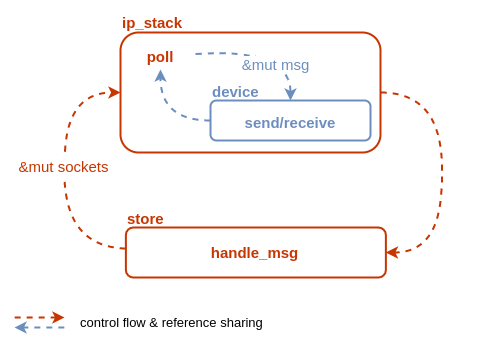
\includegraphics[height=5cm]{figures/outer_scope_before.png}
    \caption{Simplified structure of the original process loop}
    \label{fig:mainLoopOriginal}
\end{figure}

Now for this simplified structure, we can already see what needs to be done to achieve our target characteristics. We need to move the inner loop inside \rust{poll} into the main scope.
For now we assume we had simply split \rust{poll} into parts e.g. asking the \rust{device} for availability, waiting before poll, preparing packets and sending them. And we create a method \rust{ip_stack.process()}, that can execute either of those parts, based on the input.
Also we change all method signatures to explicitly return and except values instead of references.This directly results in the structure shown in Figure\ref{fig:mainLoopTarget}. 

\begin{figure}[H]
    \centering
    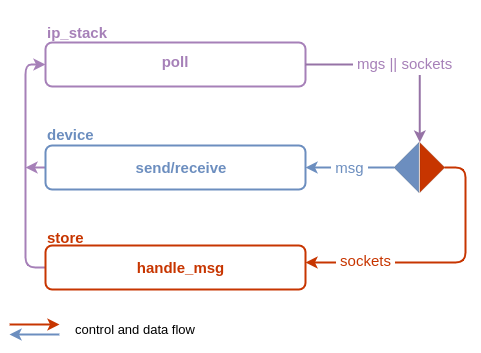
\includegraphics[height=5cm]{figures/outer_scope_target.png}
    \caption{Simplified structure of the target process loop}
    \label{fig:mainLoopTarget}
\end{figure}

Without looking at the inner workings of poll in detail, we can already recognize essential properties of the target program here

\begin{enumerate}
    \item The final structure is a nested loop.
    \item Since we want to use only one method call for the \rust{ip_stack}, it must return a type which can be either an input for the \rust{device} or the \rust{store}.
    \item The calls to \rust{device} or the \rust{store} must return a common type that \rust{ip_stack.poll} accepts\footnote{you could also return different types. However, then an additional node would be needed to convert them to a common type}.
    \item In the original structure, the \rust{device} was called inside the \rust{poll} function. Therefore, after each call to \rust{device}, the control flow automatically returned to the execution state of \rust{poll}. Now the substeps of \rust{process} are individual method calls. That means we will need a way to transfer the execution state of \rust{poll} from one call to the next. 
\end{enumerate}

In the next sections, we will first take a closer look at the control flow in poll. We will describe how to implement inner loop extraction and what problems arise when converting reference arguments to moved objects, i.e. call by reference to call by value.

\subsection{Encapsulating the Socket Handling}
\label{subsec:SocketHandling}
In sketching the target program, the first change made to the original code was to encapsulate as much of the logic as possible into either the states or the initialization functions. As a first guess, the socket handling i.e. checking if sockets are open, setting them to listening state etc. was encapsulated in the \store{.handle_sockets} call. The problem with this decision is, that the actual \rust{SocketSet} type contains lifetime bound references, meaning they do not implement \rust{Clone} and we can not just replace passing them by reference with actually moving them. Implementing a custom, owned version of the \rust{SocketSet} would be a remedy for this problem. However, the internal references are actually different buffer types used in the sockets and manipulated in many places in the core logic of smoltcp. This means that implementing a custom, owned \rust{SocketSet} type would not only result in extensive changes, but would also negatively affect the efficiency of the program. The other option is to not send the sockets, but only the required information among components. What this required information is, depends on the interaction on how either of the components involved interacts with the sockets. For our example key-value store application, the interaction between sockets and \store{} is fairly simple. The \store{} receives a message from a socket and answers it. As we will later see, the interaction between the \stack{} and the sockets is rather involved. So instead of having a free-floating \rust{SocketSet} in the main scope, we make it part of the \stack{} upon initialization. This also means, we need to move the code for handling the sockets into the \stack{} as well and return to the \store{} not directly after polling, but when a socket is processed. We will discuss how this is done in Section~\ref{}\todo[inline]{Where?!}. The main point here is to illustrate the problem of designing the interfaces between components, if they are not clearly defined in the first place. A less simple case could have involved for instance conditional opening or closing of sockets by the \store{} based on concrete messages, time, traffic volume etc. and would have required an extended message interface between the \stack{} and \store{} and potentially a replication of the sockets in both components updating each other via this interface. Such information can hardly be automatically derived, in particular from static, purely syntactic information from high-level language input code.


\subsection{Refactoring Packet Sending}
The next step is to refactor the \rust{poll} method. We need to bring the stateful usage of the \dev{} into the compile scope and create a single \emph{entry method} the three 
components use to call each other. This \emph{entry method} will internally dispatch each call to the actual method, or generally code to be called on the states.\\

The code of \rust{poll} is depicted in Figure~\ref{fig:pollCode}. The method itself contains a loop calling \rust{socket_egress} which executes sending packets to the \rust{device} and \rust{socket_ingress} which receives packets and distributes them to the \rust{sockets}. As long as there are packets send or received in each loop, \rust{poll} continues. \\

\begin{figure}[H]
    \centering
    
\begin{minted}[fontsize=\footnotesize]{rust}
pub fn poll<D>(
    &mut self, timestamp: Instant,
    device: &mut D, sockets: &mut SocketSet<'_>,
    ) -> Result<bool>
    where
        D: for<'d> Device<'d>,
    {
        self.inner.now = timestamp;
        let mut readiness_may_have_changed = false;

        loop {
            let processed_any = self.socket_ingress(device, sockets);
            let emitted_any = self.socket_egress(device, sockets);
            if processed_any || emitted_any {
                readiness_may_have_changed = true;
            } else {
                break;
            }
        }
        Ok(readiness_may_have_changed)
    }
}
\end{minted}
    \caption{Simplified code of the \rust{ip_stack.poll} method}
    \label{fig:pollCode}
\end{figure}

As we can see the \dev{} reference is passed further down into two method calls, the receiving method \rust{socket_ingress} and the sending method \rust{socket_egress}. We will start with explaining the transformations in \rust{socket_egress}, because it is structurally  more complex than \rust{socket_ingress} and therefore better suited to demonstrate all necessary transformation steps.

\subsubsection{Bringing \dev{} calls into scope}
\label{subsec:DeviceLifting}
Figure~\ref{fig:egressCode} shows how sending packets proceeds as a loop over the socket items. If a \rust{socket} can send, its \rust{socket.dispatch} method is called passing a reference to the \stack{} and the \rust{respond} closure. As our example works with TCP sockets, inside \rust{dispatch} the \rust{socket} prepares a TCP packet and passes it to the \rust{respond} closure. This closure will then try to get a sending token from the \dev{} and pass the token and the TCP packet. The token is basically a direct reference to the sending buffer of the \dev{}. Finally inside the \rust{inner.dispatch} call of the \rust{stack} will wrap the TCP packet into a network representation e.g. an Ethernet frame and directly write that packet into the device buffer using the token.\\
 
\begin{figure}[H]
    \centering
    
\begin{minted}[fontsize=\footnotesize]{rust}
fn socket_egress<D>(&mut self, device: &mut D, sockets: &mut SocketSet<'_>) 
-> bool
    /*where*/
{
    let Self {
        inner,
        ..
    } = self;
    let mut emitted_any = false;
    for item in sockets.items_mut() {
        if ! can_send(item, inner.now) {
            continue;
        }

        let mut neighbor_addr = None;
        let mut respond = |inner: &mut InterfaceInner, response: IpPacket| {
            neighbor_addr = Some(response.ip_repr().dst_addr());
            let token = device.transmit().ok_or_else(|| {
                /*logging*/
                Error::Exhausted
            })?;

            inner.dispatch_ip(token, response, None)?;
            
            emitted_any = true;

            Ok(())
            };

        let result = match &mut item.socket {
            Socket::Tcp(socket) => socket.dispatch(inner, |inner, response| {
                respond(inner, IpPacket::Tcp(response))
            }),
            // .. other socket types
        };
        
        match result {
            // stop looping if the device was exhausted
            // update socket if adress was wrong
        }
    }
    emitted_any
}
\end{minted}
    \caption{Simplified code of the \stack{.socket_egress} method}
    \label{fig:egressCode}
\end{figure}

 The \dev{} is used twice in this method. Once for receiving a token in the \dev{.transmit()} call, a second time implicitly when this token is used to pass a packet to the device. This happens inside \stack{.inner.dispatch_ip}. Both of this calls happen inside the \rust{socket.dispatch} method. If we look into this method and inline the code of the \rust{response} closure we get the following structure: 
 
\begin{minted}[fontsize=\footnotesize]{rust}
//socket.dispatch(...)
    /*check socket state*/
    if /*a packet can be produced*/{
        let packet = /*produce packet*/;
        neighbor_addr = Some(response.ip_repr().dst_addr());
        let token = device.transmit().ok_or_else(|| {
            /*logging*/
            Error::Exhausted
        })?;
        inner.dispatch_ip(token, response, None)?;
        emitted_any = true;
        Ok(())
        /* 
        if no error occured, update socket state
        using the packet information        
        */
    } else {
         return Ok(())
    }                    
\end{minted}

The method starts with a preparation phase were the socket state is checked. If no packet can be produced, the it returns with \rust{Ok(())}. If a packet is produced, a token is required and if successful the packet is send. Afterwards the socket state is updated using information from the packet. If any of the steps fail, the control flow returns an error to the outer scope i.e. to the sending loop. 

\todo[inline]{Find better Name}
\textbf{Refactoring Packet Processing}

To lift device usage into compile scope, we need to inline the content of \rust{socket.dispatch}. This means we refactor a function scope i.e. a separate stack frame to a simple scope in the outer stack frame. Scopes are expressions in Rust. So there are two different ways of returning values from scopes. One is to simply end the scope with an expression. In this case, the scope simply returns the value of that last expression to the outer scope. The second is to use explicit \rust{return} or \rust{?}. They will not only return a value or an error to the surrounding scope, but leave the current stack frame. \\

 So to inline function with early returns or \rust{?}, we need to refactor the early returns to conditional execution i.e. we need to 
 \begin{enumerate}
     \item instantiate a \rust{let result;} at the beginning of the method and whenever either a \rust{return x} or a \emph{expression}\rust{?} appears
     \item replace any returning statement including the final return by binding the potential early return values to the \rust{result} variable, in our example for instance \rust{result = inner.dispatch_ip(token, response, None);}
     \item wrap every subsequent code into a conditional and, 
     \item return the assigned \rust{result}
 \end{enumerate}
\todo[inline]{reference further details in the 'general learnings' or 'not yet supported syntax' section if I have time to spell it out}. 
Now we can safely inline the code. \\
\todo[inline]{figure for inlined code}
\todo[inline]{learnings \means refactoring early returns needed for inlining, otherwise inlined code must comply prog. mod.}

After lifting \rust{socket.dispatch} into scope, the steps before and after the device usage can be re-encapsulated into package pre-processing \rust{socket.dispatch_before} and the socket post-processing and after sending \rust{socket.dispatch_after}. Thereby we see another refactoring problem. When we split execution steps into different functions. In the original code, the 'packet' i.e. the two representations where used in emit and afterwards to update the socket without any referencing or cloning. This was possible, because they implement \rust{Copy} and can therefor be implicitly duplicated. This still works when we inline the socket.dispatch code because still any processing of the packet happens in a single, now extended stack frame. However it stops working as we re-encapsulated packet handling before and after sending. The reason is, that with that re-encapsulation the frame producing the packet (i.e. the pre-process call) is gone, when we want to send it. \\
\note{This would also happen if we did not re-encapsulate but left the code inside poll. The reason is, that in any case the steps will be interrupted by a call to the device i.e. by leaving the current stack frame}

To fix this problem, we introduced a heap-allocated version of the package data type. Also, pre-processing now returns two copies of the packet so that one can be used for sending and one for post-processing the socket. 
\note{This is a general problem when we want to make sequential code concurrent or even distributed. In the first case, types need to be transferable from one function stack. Ohua can not recognize, nor can we automatically implement something like copy, clone or serialization for 
types. Before we assumed, that arguments are always passed by value and 
that serialization in the chosen backend is available for all types used as arguments in the compile scope i.e. all types that are send among nodes later. If we tried to implement refactorings/transformations in the compiler that a) split functions or b) bring code into scope that wasn't before, we need to extend this assumption to all code possibly affected by the transformation}
\todo[inline]{figure for refactored code}
\todo[inline]{Note that this refactoring need to happen on the implementers of the socket trait individually, because we need to split concrete implementations of dispatch}


\textbf{Refactor token usage}
Now we need to eliminate the implicit use of the \dev{} inside \stack{.inner.dispatch_ip(token, response, None)}. The sending \rust{token}, passed to this method contains a reference to the \dev{}s sending buffer. So the function as it is violates two requirements by using shared references among components and using one component implicitly inside the other.
Contrary to packet processing, this method ends with the call to the device, meaning there are no state changes occurring after the sending and except the sending result, nothing depends on the actual device behavior. This means, we can separate the packet preparation inside \stack{.inner.dispatch_ip(token, response, None)}, from the effective packet sending in the device, making both steps local to their component. For the \stack{} we provided a local implementation of the sending token. Like the original token, the \rust{LocalToken} holds a reference to a buffer and implements the expected \rust{token.consume} method. Also we replaced the direct call to \stack{.inner.dispatch_ip}, by a wrapper function \stack{.inner.dispatch_local}. That function instantiates a local sending token, executes \stack{.inner.dispatch_ip} and returns the token buffer
containing the packet. On the other hand the device needs an explicit sending method, instead of an implicit call via the token. This new \dev{.send} method basically needs to call the \rust{token.consume} method on a given token, with a given packet. Therefor we do not need to have specific implementations for implementers of the \rust{Device} trait, but can implement \rust{send} directly on the trait. The method \rust{token.consume} does not take a packet, but a closure processing a packet and copying it into a given buffer. Both already happened in the \stack, so we only need a closure, that copies the given packet into the actual device buffer. Finally, with respect to our target architecture there is no particular use in requesting and returning actual tokens to the device any more. In a distributed system, file pointers as contained in the tokens can not trivially be send among components. Therefor, instead of sending tokens we only request them locally in the device when needed and send \rust{Result<()>} to the \stack{} instead. Hence the implementation of the sending function looks as follows:

\begin{minted}[fontsize=\footnotesize]{rust}
pub trait Device<'a> {
    type RxToken: RxToken + 'a;
    type TxToken: TxToken + 'a;
    // ... 
    
    fn send(&'a mut self, timestamp:Instant, packet:Vec<u8>) -> Result<()> {
        let sending_result
            // Request a token locally
            = self.transmit().ok_or_else(|| {
                        net_debug!("failed to transmit IP: {}", Error::Exhausted);
                        Error::Exhausted
                    }).and_then(|token|
                    // copy the packet to the devices sennding buffer
                   token.consume(timestamp, packet.len(),
                     |buffer| Ok(buffer.copy_from_slice(packet.as_slice()))));
        sending_result
    }                 
\end{minted}

\note{The functional split between device and \stack{} can hardly be derived  automatically and in particular statically. Actually I don't think its possible. What needs to be understood by the compiler is 1. there are no state changed in the interface depending on the device reaction 2. tokens contain references to the device i.e. to buffers, file pointers etc. 3. we can split the closures passed to token\_consume into 'preparing a packet and copying it to a local buffer' and 'copying it to the actual buffer'. We also can not just send the closures. What might be possible is to 1. analyze what arguments from the ipstack the closure takes, 2. send those arguments to the device and 3. have the actual closures stored as functions in the device and execute them. Not quite clear if this would work ... Device would need to know which closure to execute, what happens if they are nested etc. pp.}

\subsubsection{Refactor to Message Passing}

We inlined the code for \rust{socket_egress} into \rust{poll} and lifted the usages of the \dev{} into the scope of the \rust{poll} function. This also means that the control and data flow for sending are now explicit in the \rust{poll} function. Figure~\ref{fig:egressInlinedFlow} shows the principle structure of the sending loop at this stage. The actual code at this point can be found in the Appendix~\ref{appFig:egressInlinedOriginal}. As indicated by dashed and solid errors in the graph, the control flow and the data dependencies of the individual steps are not congruent. In particular the currently processed \rust{socket} is needed in multiple steps in the \stack{}, but not needed by the \dev{}. 

\begin{figure}[H]
    \centering
    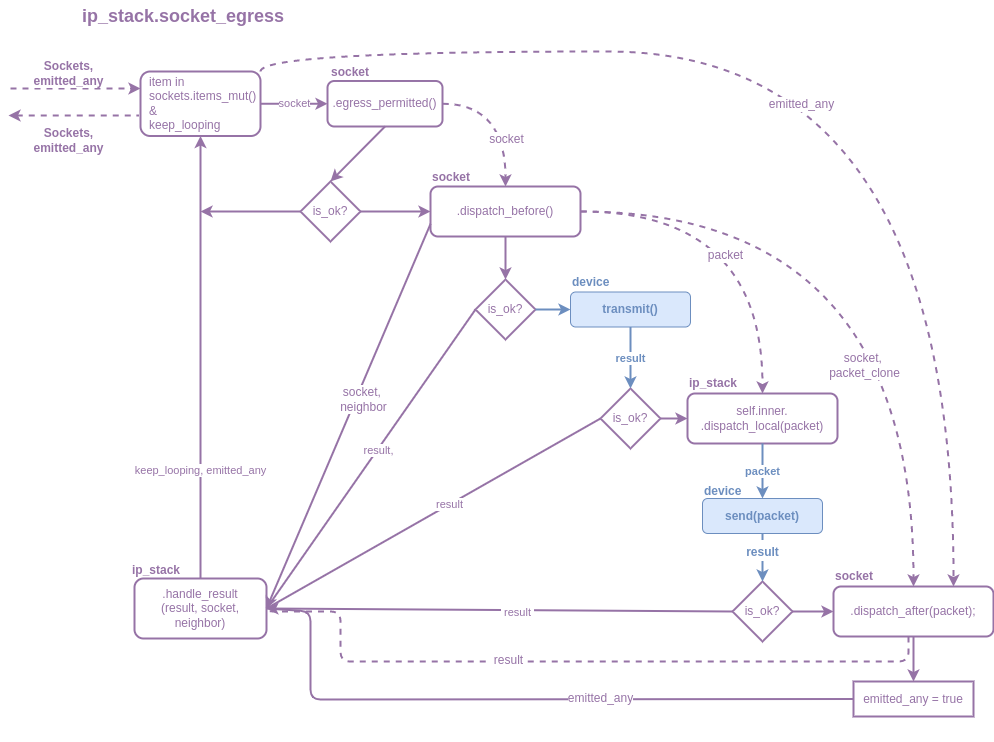
\includegraphics[scale= 0.36]{figures/egress_inlined_detail.png}
    \caption{Structure of the packet sending loop after lifting all device usages into scope. 
    Solid arrows indicate actual control flow, dotted arrows indicate data dependencies}
    \label{fig:egressInlinedFlow}
\end{figure}

\textbf{Refactoring control flow}

Currently the sending loop happens entirely inside or above the stack frame of \rust{poll}. That's why is is possible to use data references and resume execution automatically after the \dev{} is called. We need to refactor the loop such that it is possible to return to the frame of the main function when the \dev{} is called and resume the execution inside the \stack{} afterwards. As method calls of the two components are interleaved, we can not just merge the calls of each component i.e. call the \stack{} to get a packet, call the \dev{} to send it and modify the \stack{}s state again based on the \dev{}s response\footnote{Actually this is an opportunity if state changes in each component are either idempotent or ordered i.e. implemented as Conflict-Free Replicated Data Types. Both is not the case here.}. This necessarily means, we need to split the execution of \rust{poll} into several method calls and we need to preserve the state of execution and the state of variables inside \rust{poll} from one sub-call to the next. 

When we split the \stack{.poll} method, or in general any method into separate \emph{sub-methods}, we have two options to transfer data from one call to another. One is pass them explicitly, the other one is to make them part of the state. Serialization is generally expensive and also in terms of security and process isolation, it is desirable to only send data around that is actually needed in other components. Analyzing the data dependencies between the \stack{} and the \dev{} it is obvious, that the only arguments the \dev{} calls require are the packet to send and in the actual implementation a timestamp and the length of the packet. So except for the packet no data needs to leave the \stack{} towards the \dev{}. We will therefor only integrate the packet into the explicit data flow, and preserve the state of other variables in the state of the \stack{}.\\

A common obstacle in both data handling options is the elimination of reference usage. As explained in Section~\ref{subsec:Rust} Rusts Type system will point to a problem, when we try to share references among different stack frames. By splitting the original \stack{.poll} method, we execute code that was supposed to run in one stack frame in multiple frames. This means we can not simply use the data types of the original program. In particular, regardless if we send data or store them in a state between function call, they must not use references among each other. This is obvious for serialized data, as references serialized and send to processes potentially running on a different machine loose their relation to memory. For the case of data stored in a state, consider the following example from our problem. The sending loop is an iteration over the \rust{sockets}. So at the point, where a packet is produced, there are four references to the same memory location in scope namely i) the sockets ii) the iterator on the sockets iii) the current socket and iv) the packet, which actually is a reference to memory inside the socket until it is finally send. As mentioned before, packets need to be become an owned data type to be sendable to the \dev{}. Which eliminates the fourth reference. However we also need to store the state of iteration and the current socket in the state, without references to the sockets. It is in general not possible to return a \rust{struct} with fields referencing each other in Rust, because the consistency of references can not be guaranteed\footnote{Actually there are ways to achieve memory consistency across function calls in Rust using e.g. the \rust{std::pin} module. However they are not applicable to other languages so we do not consider them here.}. In particular we can not have a socket, referencing an iterator, referencing the sockets in our current state, since any of those reference could become independently invalid leaving dangling references. \\

The problem was solved by implementing an owned representation of the iteration state. As shown in, we integrated the current state of \stack{.socket_egress} as a separate, optional field to the \stack{}. Instead of saving an iterator and a reference to the current socket, only an index of the current socket in the socket set is stored. The socket itself must be retrieved in ever step using it. This also implied, that we need to rewrite the iteration on the socket set. Instead of using the given \rust{Iterator} implementation, we implemented iteration over the size of the socket set, starting at the currently saved index. We did the same for the other intermediate results of the original method \rust{neighbor} and \rust{packet} and \rust{address}. The resulting definition of the \stack{} data type is shown below. 

\note{What we can learn here are two things a) a lambda lifting for method may include turning enclosed values to part of the state instead of explicit arguments and b) as long as the compiler is not smart enough to transform references to owned data (which has quite some implications on the code structure) we need to extend the requirement of 'no shared refs, no calls on refs, no refs anywhere in scope anyway' to all the code the compiler might touch.}

\begin{minted}[fontsize=\footnotesize]{rust}
struct Interface<'a> {
    ..,
    egress_state: Option<EgressState<'a>,
}
struct EgressState<'es>{
    sockets_during_egress: Option<SocketSet<'es>>,
    current_index: Option<usize>,
    current_neighbor:Option<Address>,
    current_presend_packet: Option<IpPacketOwned>,
    current_postsend_packet:Option<IpPacketOwned>
}
\end{minted}

Now the control flow needs to be refactored, such that the device is called in the main scope and \dev{} and \stack{} have each only one method call visible to the compiler. This method will be \emph{entry point} of both states and internally dispatch the call to the required code. We will call the method \rust{process_call} and start by defining it on the \dev{}. \\

Intuitively \rust{process_call} would be a higher-order function. Specifically, instead of calling the \dev{} directly, \rust{poll} would return the functions \rust{transmit} or \rust{send} including the necessary arguments. The device would then be called with \dev{.process_call(fn, [args])}. However higher-order functions are not a viable solution here. This is for two reasons. Firstly we envision to send the functions to be called by \rust{process_call} from one component to the other. But function references are, with some exceptions, not serializable and sendable in distributed scenarios. Secondly we also need to pass the arguments for those called functions to \rust{process_call} so we would need to derive a common sum type to represent all possible function arguments.

The solution to this is called defunctionalization. It is a known transformation used in compilers to transform higher-order functions \cite{reynolds1972definitional}. Instead of sending function references, a sum data type representing all possibly called functions is defined. In Rust we can use \rust{enum}s for this purpose. This \rust{enum} data type also allows us to integrate the arguments called per function so the \rust{enum DeviceCall} looks as follows for the sending loop: 
\begin{minted}[fontsize=\footnotesize]{rust}
#[derive(Debug, Eq, PartialEq, Clone)]
pub enum DeviceCall{
    Transmit,
    Consume(Instant, Vec<u8>),
}
\end{minted}

We merge control flow and data flow here so the return type will be the union of the return types of all functions that might be called, wrapped in the respective next step of execution. In case of the \dev{}, the next step of execution will be a the next part of the \rust{poll} function to be executed. Therefor we define \dev{.process_call} as follows:
\begin{minted}[fontsize=\footnotesize]{rust}
pub trait Device<'a> {
    // ...
    
    fn process_call( &'a mut self, call: DeviceCall
    ) -> InterfaceCall
    {
        match call {
            DeviceCall::Transmit
                => InterfaceCall::InnerDispatchLocal(self.transmit()),
            DeviceCall::Consume(timestamp, packet)
                => InterfaceCall::MatchSocketDispatchAfter(self.send(timestamp, packet)),
    }
}
\end{minted}

In principle, each \dev{.process_call} now returns a continuation in the \stack{}.\\

For the \stack{}, the implementation of \rust{process_call} and the \rust{enum InterfaceCall} is slightly more involved. Contrary to its implementation on the \dev{}, the \stack{.process_call} method will need to call sub-sections of the the \stack{.poll} method. We will consider the simplified pseudocode version shown below for now, to illustrate the principles applied. In the code below, borders of basic blocks, i.e. points the control flow could jump to are marked and given names, because they are needed for the transformation. 

\begin{minted}[fontsize=\footnotesize]{rust}
impl Interface {
    // 1st jump => InitSimplePoll
    fn simple_poll(&mut self, sockets: &mut SocketSet, device: &mut Device) -> bool {
        let mut something_changed = false;
        let mut result: SmoltcpResult<()>;
        // Jump here 2nd => StartSendLoop
        for socket in sockets {
            // Jump here 3rd => GetNextPacket
            let next_packet = self.maybe_get_packet(socket);
            if next_packet.is_ok() {
                result = device.send(next_packet);
                something_changed = result.is_ok();
            } else {
                result = next_packet.as_err()
            }
            // Jump here 3rd => HandleResult
            self.handle_result(result)
        }
        something_changed
    }
}
\end{minted}

Now the transformation from \stack{.simple_poll} to \stack{.process_call} would proceed as follows. First the basic blocks are identified. From those blocks, a corresponding \rust{enum InterfaceCall} is defined representing each of them. If a block uses results from the \dev{}, this results are part of the constructor of its \rust{InterfaceCall} representation. For our simple example this would yield the following \rust{enum}:

\begin{minted}[fontsize=\footnotesize]{rust}
enum InterFaceCall<'a> {
    InitSimplePoll(SocketSet<'a>),
    StartSendLoop,
    GetNextPacket,
    HandleResult,
}
\end{minted}

The \stack{.process_call} is again essentially a \rust{match} expression on the given call. The arms of the matches wrap the respective parts of \rust{simple_poll}. The next modification we need, is to augment every such arm with statements to restore the original environment of each block inside the match arm. We stored the variable state inside the state of the \stack{} as described before, in this trivial example we assume to set them directly as filed of the \stack{}. However the code in the branches might still use references to the variables and we need to respect rusts borrowing rules, so we can not generally replace any direct variable use \rust{f(x)} by \rust{f(self.x)}. So we add statements to get and set the stored variables in each block before the code and before each \rust{return} statement respectively. Finally we replace calls to the device by statements returning the respective \rust{DeviceCall} and jumps to other blocks by the corresponding call of \stack{.process_call(next_block_call)}. The actual return statement of \rust{simple_poll} remains unchanged. So the return type of this simplified \stack{.process_call} is \rust{Either<DeviceCall, bool>} and looks as follows. 

\begin{minted}[fontsize=\footnotesize]{rust}
    fn process_call(&mut self, call: InterFaceCall) -> Either<DeviceCall, bool> {
        match call {
            InterFaceCall::InitSimplePoll(sockets) => {
                // set variables something_changes, result, sockets and index
                return self.process_call(StartSendLoop)
            },
            InterFaceCall::StartSendLoop => {
                // get socket and socket_index
                if socket_index+1 < sockets.size() {
                    let socket_index = socket_index+1;
                    // set sockets and socket_index
                    return self.process_call(GetNextPacket);
                } else {
                    // set sockets and socket_index
                    return Either::Right(self.something_changed);
                }
            },
            InterFaceCall::GetNextPacket => {
                let next_packet = self.maybe_get_packet();
                    if next_packet.is_ok() {
                        return Either::Left(DeviceCall::Send(next_packet))
                    } else {
                        self.result = next_packet.as_err();
                        return self.process_call(HandleResult)
                    }
            }
            InterFaceCall::HandleResult => {
                self.handle_result();
                return self.process_call(StartSendLoop)
            }
        }
    }
\end{minted}

The actual implementation of \stack{.process_call} is obviously more complex, but was build in the same transformation steps. 

\todo[inline]{Find better title or reorder}
\subsection{Refactoring Packet Receiving -- Completing the \rust{poll} loop}
Just like sending, receiving is triggered in the \stack{.poll} method. The main aspects of \stack{.socket_ingress()} are depicted in Figure~\ref{fig:socketIngressCode}. In a while loop, the \stack{} tries to receive packets from the \dev{}. In this case packets are represented by a token pair. The receive token \rust{rx_token} contains a buffer holding the received packet, the send token \rust{tx_token} may be used to directly return an answer to the \dev{}. During initialization, the transport medium used by the \dev{} is saved in the \stack{}. By matching on the current transport medium the method to unwrap the outer most layer of the packet is determined, in this case \rust{process_ethernet(sockets, &frame)}. Using the reference to the sockets the function determines which socket the packet should be dispatched to. Next packet is processed by the socket and copied into its receive buffer. From there it can later be retrieved and passed to the \store{}. The socket may also produced a direct answer, for example as part of the TCP protocol. If so this answer is dispatched as discussed before for the sending loop using the \rust{tx_token} as a reference to the device. So in essence the \dev{} is used three times here. First time explicitly for receiving, the second and third time implicitly by accessing its receiving and sending buffer via the tokens.
\begin{figure}[H]
    \centering
\begin{minted}[fontsize=\small]{rust}
fn socket_ingress(&mut self, sockets:&mut SocketSet) -> bool {
    // ... 
    while let Some((rx_token, tx_token)) = device.receive() {
        if let Err(err) = rx_token.consume(inner.now, |frame| match
            inner.caps.medium {
                Medium::Ethernet => match inner.process_ethernet(sockets, &frame) {
                    Ok(response) => {
                        processed_any = true;
                        if let Some(packet) = response {
                            if let Err(err) = inner.dispatch(tx_token, packet) {/*log Send Error*/}
                        }
                        Ok(())
                    }
                },
                /*handle  other Medium types*/
            }) else {/*log Handling Error*/;
            }
        processed_any
    }
\end{minted}
    \caption{Simplified code of the \rust{Interface.socket_ingress()} method}
    \label{fig:socketIngressCode}
\end{figure}

Again we need to eliminate the use of common references between \stack{} and \dev{} and integrate the receiving control flow into the \rust{process_call} logic of both components. So we first eliminate the use of reference tokens. A packet can no longer be received via a reference to the \dev{}, hence we implement a new receiving method on the \dev{}. This new method \dev{.receive_token_free} first executes \dev{.receive}. Receiving might or might not succeed, so it needs to return an \rust{Option<Tokens>}. If token tuple is returned, an owned buffer is allocated and \rust{rx_token.consume} is called to copy the received data into that owned buffer. Instead of returning an \rust{rx_token} and a \rust{tx_token}, \dev{.receive_tokenfree} then returns the received data and simple result representing the \rust{tx_token} (i.e. \rust{Ok(())} or \rust{Error}). Consuming the \rust{rx_token} might return an error that needs to be logged in the original code, however this error can only occur during processing the \stack{} so \dev{.receive_tokenfree} does not need to additionally the result of consuming. 
Inside \stack{.socket_ingress} the usage of the \rust{rx_token} can now be replaced by simply passing a reference to the token to \rust{inner.process_ethernet(sockets, &frame)}. If a response is returned, we use the same mechanism as in the sending loop before. A local token is passed to \stack{.inner.dispatch} and the \dev{.send} function is used to explicitly send this owned token buffer to the device.

After this refactoring, the core control flow between the two components looks as follows:
\begin{minted}[fontsize=\footnotesize]{rust}
fn pseudo_ingress(&mut self, device: &mut Device) -> bool {
    while let Some(packet, send_permission) = device.receive_tokenfree() {
        let local_tx = /*init LocalToken*/;
        match inner.caps.medium {
            /*process &packet and local_tx as tokens before*/
        }
        if local_tx.len != 0 {
            let packet = local_tx.take_buffer();
            if let Err(e) = device.send(packet) {
                /*log Send Error*/
            }
        }
        
    }
}
\end{minted}

There are now two explicit, stateful usages of the \dev{} and we can apply the same procedure as with the \stack{.socket_egress} function, to integrate the basic blocks of \stack{.socket_ingress} into the \stack{stack.process_call} matching. The method itself is divided into three additional \rust{InterFaceCall}s i) \rust{InitIngress} to trigger the ingress call including the first receive call to the device, ii) \rust{ProcessIngress} handling either a received packet or ending ingress and iii) \rust{LoopIngress} logging the device result and calling the \dev{.receive} again. For the \dev{} we also needed to add two calls. One is obviously \rust{DeviceCall::Receive}. The second one is needed, because the call \rust{DeviceCall::Send}  is now used in two different control flow states of the \stack{}, once during egress and once during ingress. So we need a way to distinguish in the \stack{} if the control flow should continue in the egress or the ingress loop after a \dev{.send} call. There are at least three options to handle this, The first is to create a new \rust{DeviceCall}, the second is to save the current state in the \stack and add an additional dispatch based on this state, the third one is to make the current state another value in the data flow and have the device decide which \rust{InterfaceCall} to return after sending. We decided to use the third option and augmented the \rust{DeviceCall::Send(Packet)} with an additional parameter \rust{enum InterfaceState} being either \rust{Ingress} or \rust{Egress}. The device would now also pattern match on this parameter and return the next call to the \stack{} accordingly.

Now there is one missing element in the basic loop. In Section~\ref{subsec:SocketHandling} it was described, that the socket handling, i.e. setting sockets to listening state, calling the receive function on the socket etc. had to be moved into the \stack{} code. To simplify previous explanations we ignored this so far. If we left the socket handling in scope, the main loop would be structured as shown below

\begin{minted}[fontsize=\footnotesize]{rust}
    let mut ip_stack_call = InitPoll;
    loop {
        let device_or_app_call = ip_stack.process_call(ip_stack_call);
        if calls_dev(&device_or_app_call){
            ip_stack_call = device.process_call(device_or_app_call);
        } else {
            let socket = sockets.get_mut(socket_handle);
            /*first socket state handling */
                let outbytes = store.handle_message(input);
                socket.send_slice(outbytes);
            /*second socket_state_handling 2*/
        phy_wait(/*...*/);
        }
    }
\end{minted}
We can see that socket handling happens in two parts. One directly after the \stack{} returned from polling, the second after the \store{} is called. Therefore as socket handling was moved into the \stack{}, only one new \rust{InterfaceCall} was introduced. The first part of socket handling was directly attached to the match arm of the last \rust{InterfaceCall} during polling. Instead of only returning the polling result, the closure ending poll now also returns the request if the socket received one. The second part of socket handling was moved to a separate \rust{InterfaceCall}, capturing the result from the \store{}. This also meant, that waiting before the next poll i.e. the \rust{phy_wait} call now happens between two \stack{} calls and needs to change its position in the loop. In transforming \rust{phy_wait}, aspects had to be taken into account that have not been addressed so far. Therefore, this will be considered separately in the next section.

\subsection{Integrating the \rust{phy_wait} Call}
\todo[inline]{I need a better title for this section}
Now we need to refactor the \rust{phy_wait} call. This function is basically a wrapper function to the system call \rust{libc::select}. It accepts a file pointer and a waiting  duration and halts the current thread until either the file becomes available or the waiting duration is exceeded. The file pointer is a pointer to the system file the device uses to write the packets to. The maximum waiting duration is determined by the \rust{ip_stack} based on the current state of sockets. We are facing two problems with this function. One is, that we need to integrate it into the refactored control flow. The second is, that it is using a system call and a file pointer. Both file access and system calls are operating system specific, and therefore may be implemented differently in m3 or any other target architecture. 

Functionally, three things are realized in the \rust{phy_wait} call. Determines the maximum waiting time for the sockets is obviously a reading operation on the state of the \stack{} and should be integrated in \rust{ip_stack.process_call}. Determining the file pointer availability in a distributed setting needs to happen in the component that holds the pointer, so we will need another call to the device. Finally waiting is a system operation. The component that should wait is the interface. However we need to implement waiting in an m3 specific manner and therefor we either have to do it in the main scope, or we have to import the according m3 API into the \rust{interface} module. The clearly preferable option is to wait in the main scope over mixing component internal logic and runtime logic. So in essence wwe refactor the \rust{phy_wait} call to another loop between the \stack{}, the \dev{} and the main scope\\

As waiting should always happen immediately after 'loading' the sockets with answers to their requests, we do not need to introduce another \rust{InterfaceCall}. We rewire the internal logic of \rust{ip_stack.process_call}. So far we just ignored waiting. After the sockets are loaded with messages from the store in \rust{ip_stack.process_call(AnswerToSocket(Vec<(SocketHandle, Vec<u8>)>)}, we would directly proceed calling \rust{self.process_call(InitPoll)} again. Now instead the waiting time for the sockets is calculated as it was in the main loop using the \rust{self.poll_delay()} function. Then the calculated duration is send to the device using a new \rust{DeviceCall}. \\

To process the new \rust{DeviceCall::NeedsPoll(Duration)}, we define a method \rust{needs_poll} on the device trait. \md implemented its network stack with smoltcp, but provides altered versions of the devices. Those devices provide the \rust{needs_poll} method to implement waiting in the main scope, so this refactoring mimics their behavior while allowing us to run our refactored smoltcp version also on standard Linux. The method accepts a duration and returns a boolean indicating if the device is available again. In the concrete implementations of the device trait we can again use \rust{phy_wait}, to maintain original behavior while we do not run on \md. \\

Finally we need to alter the general control flow. Waiting has to happen in the main scope in \md. So after calling the \dev{} with \rust{DeviceCall::NeedsPoll}, the \stack{} should not be invoked directly as before but instead a waiting function is called, mimicking the behavior of \md waiting implementation. This means a call to the \dev{} can now either return a call to the \stack{} or an instruction to wait, containing the information \md will require for waiting. Consequently in the main scope a new case distinction is needed. If the \dev{} returned an \rust{InterfaceCall}, it is directly forwarded to the \stack{}, otherwise the waiting instruction is executed by a placeholder and and the \rust{InterfaceCall} to restart polling is generated. TO keep control flow simple in the main loop, this case distinction is wrapped in a function \rust{maybe_wait}, yielding a control flow as shown the pseudocode below

\begin{minted}[fontsize=\footnotesize]{rust}
    loop {
        let device_or_app_call = ip_stack.process_call(iface_call);
        if is_device_call(&device_or_app_call){
            let iface_call_or_wait = device.process_call(device_or_app_call);
            iface_call = maybe_wait(call)
        } else {
            // call the store to answer messages
        }
    }
\end{minted}

\section{Adaptations in Ohua}

Although Rust is a strongly typed language, type annotations for local variables are often unnecessary, since they are automatically derived from the type inference of the rust compiler. In contrast, definitions of types, i.e. structs, enums and functions, are the basis of type inference and must be annotated manually/by the programmer. Since Ohua produces new code in the backend, it is not enough to transfer existing annotations of the input to the output. In particular, the communication channels of the produced tasks require type annotations, since these cannot be completely derived by the Rust type inference even in the shared memory scenario. Also in view of a later extension to fully distributed systems, distributed compilation of individual components or the use of languages with less powerful inference, it is important not to rely on the type inference specific to the compiled language. 

So where do we get the type information we need? One important observation is that Ohua does not create new types. The control functions Ohua inserts into the data flow graph are mainly there to pass on existing intermediate results of the original program. That is, the types of these functions that is, of their input and output channels can be derived from the input code. For this we need a) a type extraction from the input program and b) a type propagation which propagates the corresponding types through the representation of the data flow graph. Both were basically available at the beginning of the work. However, the existing implementation had problems or was not fully functional. This means that some types had to be annotated by hand in the output code. The following sections describe how type extraction and type propagation worked and which changes were necessary to achieve the desired functionality. \\

\subsection{Type Extraction}
So the first functionality we had to address was the \code{Type Extraction} in the frontend integration. Until now this was a two step process. In a first pass two kinds of data were extracted from the input module. One was the algorithms i.e. the Rust functions that were to be compiled. Those were translated to an internal representation of the supported Rust subset as described in Section~\ref{subec:OhuaPipeline}. The second structure kept track of imports defined in the module. \\

The second pass was needed to annotate types to function names. As each function call \rust{let z = someFun(x, y);} might become an independent node, the compiler needs type annotations for \rust{x} and \rust{y} to later annotate the channels for sending those variables among independent tasks. To do so first the function names called in the parsed algorithms were extracted. Then all files defined in the imports where scanned for function definitions. From this information, a hashmap was built over all function names and the extracted function types. Finally, in a further traversal over the input code, this hashmap was used to lookup function types and annotate them in the input code. This procedure had some disadvantages, namely : 

\begin{itemize}
    \item The entire compile scope, including for example the standard library, had to be available for the compiler to find and process. This introduced path dependencies of the compiler and notably excludes the import of compiled libraries in other languages e.g. libc, which is critical in our case.
    \item We had to restrict the entire compile scope and imported libraries to syntax the compiler could understand. This has previously been addressed by re-implementing some required libraries in a simpler form. 
    \item We had to keep track of name spaces and aliasing for all functions
    \item We could not support 1. generic type parameters in function definitions and 2. overloaded function definitions.
\end{itemize}

The main point of concern was really the need to parse the whole scope and therefore to have all libraries used available and compatible to Ohua supported syntax. Therefore we chose to change the source of type information. Instead of collecting function signatures from the scope and typing functions globally for the complied module, we now type each call site according to the local context. Remember, we need to type the input parameters for each function call inside an algorithm. Those parameters can be: 

\begin{itemize}
    \item global constants, in which case Rust requires a type annotation
    \item input parameters of the algorithm, in which case we know their type from the algorithm signature
    \item local variables bound in the algorithm, in which case we now require the programmer to provide type annotation 
\end{itemize}

So for most syntax constructs, we can derive the type information needed from the local context. This requires the programmer to annotate types manually in local assignments, where it would not be required by Rust itself. Also Figure~\ref{fig:TypeExtractionExample} shows an example, where additional local bindings are required. In the example code, to be able to type the function call to \rust{h(e)} we need an additional binding statement as it is not possible to type annotate a loop pattern currently. 

\begin{figure}[H]
\centering
\tabskip=0pt
\valign{#\cr
    \hbox{%
    \begin{subfigure}{.35\textwidth}
    \centering
     \begin{minted}[fontsize=\footnotesize]{rust}
fn test(i:i32) ->  {
    let s = State::new();
    for e in range_from(i) {
        let r = h(e);
        s.some_method(r);
    }
    s
}
     \end{minted}
    \end{subfigure}%
  }
  \cr
  \noalign{\hfill}
    \hbox{%
    \begin{subfigure}{.62\textwidth}
    \centering
    \begin{minted}[escapeinside=||,fontsize=\footnotesize]{haskell}
fn test(i:i32) -> () {
    let s:State = State::new();
    for e in range_from(i) {
        let e1:i32 = e;
        let r:i32 = h(e1);
        s.some_method(r);
    }
    s
}
    \end{minted}
    \end{subfigure}%
  }
  \vfill
  \cr
}
\caption{To extract type information for function call from the local context we require the  programmer to annotate the according types to local variables. As shown in the right code example it is sometimes also necessary to have additional binding statements to annotate every relevant variable i.e. every input to a function call.}
\label{fig:TypeExtractionExample}
\end{figure}

However, the new \code{Type Extraction} works without the need to parse the imported files. As we only type the concrete function call sites, this also allows the use of generically typed.\\
\todo[inline]{Check with felix whether and how this was a problem anyways since Ohua is perfectly fine with generics and also Rustwise it should be ok to infer at compiletime as usual}

The main change, required to implement this solution was threading a monadic context through the complete process of transforming the input code to the frontend representation. In particular also through the first step of this process, where the Rust code is mapped to a subset of Rust supported by Ohua. These context keeps track of variable bindings and according types in the current scope. In the outermost scope i.e. the global level of the input code, this context is pre-filled with constant definitions, including all global constant definitions parsed before the actual algorithms. 

The conversion of algorithms is also monadic process and the initial context contains the names and types extracted from the global scope. For each algorithm the parameter names and their types are parsed from the signature and added to the context. Upon parsing the body of the algorithm each right hand side of a let binding\footnote{We currently only support variable or tuple patterns} is checked for type annotation and registered in the local context if annotated properly. Unannotated bindings will yield an error at this point. AS shown in the example in Figure~\ref{fig:TypeExtractionExample} this might require some additional local assignments, when local variables result from pattern binding.\\

Now, whenever a function call is converted, the function type is derived from its arguments. In the case of a stateful call, this also includes the called object. If the arguments are variables, the types are obtained from the context. If the variables are not in the context, again an error is thrown. For supported literal arguments (currently integers, booleans and strings) the types are derived automatically. Obviously, this limits the accepted input syntax in that only literals and variables are valid as direct function arguments. Still the advantage of being able to use the entire Rust syntax again in the imported libraries outweighs this in our opinion. As function types now depend on the types of local variables we added test cases to the regression test suite to ensure proper typing, when local scope variables shadow names from outer scopes. Notably name shadowing is currently only supported for loop local scopes.  Ohuas renaming algorithm and could therefore not be tested.\\

\todo[inline]{Check where the below comments belong}
\note{Finally there are some open question we need to address regarding accepted types. Currently the type extraction mechanism just wraps any relevant type annotation from the input code in a to an internal argument type representation. This means, we do not distinguish the actual Rust types and do not filter for references, pointer or trait objects. The goal is of course to develop Ohua and the programming model for Rust to the point where a valid sequential input program never leads to an invalid output program, i.e. we want to achieve soundness. For this we need to evaluate if and how the type system of Rust has to be restricted in the input. And so we need to decide whether to leave this to the programmer, because it depends for example on the chosen backend or if there have to be additional mechanisms in the compiler to enforce these restrictions. We might also need to extend the programming model by necessary augmentation on the original program, like additional trait bounds. For example, an automatic annotation with \rust{[\#derive]} could be generated to add traits, e.g. for serialization, that were not necessary in the serial program. We will consider those question in the further development of Ohua and in particular the Rust integration.}

\subsection{Type Propagation}
The second aspect arises in the core compiler. When Ohua generates a Data Flow Graph, it introduces control functions e.g. to guard branching or collect results of a loop (see \ref{} for further details). Some of those functions are only present in intermediate representations because node fusion implemented downstream in the compiler may integrate them into bigger nodes. Some however occur as separate tasks in the final program. In particular for the later kind, proper type annotations are essential but it is sensible to provide them for any such function if possible, to reduce the assumptions among the steps of compilation. Also the transformation of code to SSA form introduces new variable names that need to be typed.\\

Control function by their nature do not introduce new types. So it is possible to infer most of their input and output types from the host-language types parsed in the frontend. The code example in Figure~\ref{fig:TypePropagationExample} shows a Rust function and its last representation in the compilers \code{DFLang} representation. Marked in $\mathbf{bold}$ we can see the functions Ohua introduced to control the dataflow in the final program. We can also see, that one of those functions, namely $\mathbf{smap}$ is not preceded by the namespace marker $\mathbf{ohua-lang/}$. This is because most of the control functions are currently not represented by own constructors of the function representation in \code{DFLang}. They are represented internally just the same as host-language function calls and only recognized in pattern matching upon their names. In contrast $\mathbf{smap}$ is already implemented as a separate constructor. 

\begin{figure}[H]
\centering
\tabskip=0pt
\valign{#\cr
    \hbox{%
    \begin{subfigure}{.35\textwidth}
    \centering
     \begin{minted}[fontsize=\footnotesize]{rust}
fn test(i:i32) -> () {
  let s:State = State::new();
  for e in range_from(i) {
     let e1:i32 = e;
     let r:i32 = h(e1);
     s.gs(r);
  }
}
     \end{minted}
    \end{subfigure}%
  }
  \cr
  \noalign{\hfill}
    \hbox{%
    \begin{subfigure}{.62\textwidth}
    \centering
    \begin{minted}[escapeinside=||,fontsize=\footnotesize]{haskell}
    let s_0_0_1 = 
        |$\mathbf{ohua.lang/unitFun}$|(State/new_state, ()) in
    let a_0_0 = /range_from ($i) in
    let (d_1, (ctrl_0_0, ctrl_0_1), size_0) = 
        |$\mathbf{smapFun}$|(a_0_0) in
    let s_0_0_1_0 = 
        |$\mathbf{ohua.lang/ctrl}$|(ctrl_0_0, s_0_0_1) in
    let lit_unit_0 = 
        |$\mathbf{ohua.lang/ctrl}$|(ctrl_0_1, ()) in
    let r_0_0_0 = /h (d_1) in
    let (_, ) = /gs [s_0_0_1_0] (r_0_0_0) in
    let d_0_0 = 
         |$\mathbf{ohua.lang/unitFun}$|(ohua.lang/id, lit_unit_0) in
    let x_0_0_0 = 
        |$\mathbf{ohua.lang/collect}$|(size_0, d_0_0) in
    let c_0_0 = |$\mathbf{ohua.lang/seq}$|(x_0_0_0, ()) in
    c_0_0
    \end{minted}
    \end{subfigure}%
  }
  \vfill
  \cr
}
\caption{Example of a Rust input function and its last stage in the core compiler representation DFLang. Functions in $\mathbf{bold}$ are control functions, introduced during compilation that need to be type annotated.}
\label{fig:TypePropagationExample}
\end{figure}


Basically, the \code{Type Propagation} works as follows. Remember in the frontend we annotated the argument types for the called Rust functions, in the example in Figure~\ref{fig:TypePropagationExample} the function calls \rust{State::new_state()}, \rust{range_from(i)}, \rust{h(e1)} and \rust{gs(r)}. Using this information the type propagation happens in a bottom-up traversal over each compiled algorithm. Due to this bottom-up processing each use of a variable is processed before its assignment. That means in our example, the function call \rust{(_, ) = /gs [s_0_0_1_0] (r_0_0_0)} is processed before the assignment \rust{r_0_0_0 = /h (d_1)}. As the function call is processed its argument types are used for two things 1. update the type field of the variables used in the call and 2. update the context to contain the associations between the variable names and the according function type arguments. \\

Contrary to Rust function calls argument types of Ohua control functions are not annotated at this point. However we can always tell their output type from the input, because they only guard data flow and do not calculate results themselves. For example the \code{collect} control function is introduced to collect the results of a loop. We know its signature has to be \code{collect:: nat -> A -> [A]}, to collect a given number of arguments of type \code{A} before returning a list of type \code{[A]}. If the output list is used by another function downstream, we already know the type \code{A} from the context and can completely annotate the variables in statements using \code{collect}.\\

Now there were two problems with the existing implementation of the \code{Type Propagation}. The first rather trivial one was, that several control functions where not or incorrectly processed. The second problem is illustrated in the  code example. It is possible that a graph ends in one or more control functions. In this case there output is not used by any typed Rust function, so we could not type there arguments and returns in the bottom up pass. Due to this problems, the existing \code{Type Propagation} was only partially functional. While the former \code{Type Extraction} mechanism just complicated or restrained the assembly of proper input code, missing \code{Type Propagation} functionality actually leaded to non functional code, in the sense that type annotations had to be made manually in the output code after compilation.  \\

To fix this issue we have made two main changes. First, we have extracted the return type for all algorithms, i.e. all compiled functions in the frontend. This is now passed as an additional parameter through the compiler pipeline and is available in the type extraction. In the example code in Figure~\ref{fig:TypePropagationExample} the return value is \rust{c_0_0}. Given this type information we can now also annotate Ohua control functions whose output is not used by an annotate Rust function in the bottom-up pass. The second change was obviously to fix or add type propagation for previously wrongly typed control functions. Finally all tests where adapted to expect correct typing of the output code. \\

One problem that has not been addressed in this work is that the control functions are not represented by separate constructors in the DFLang. This means that they can only be distinguished from normal Rust functions by their function name, which is error-prone and difficult to maintain. So in the future the control functions should at least be mapped in their own constructors. Also arguments with known type, like the first argument of the function \code{collect:: int -> A -> [A]} should optimally be enforced by the type system. 

\subsection{Destructuring Higher Arity Tuples}

Destructuring of function output was limited to to flat tuples of two elements. As shown in the Example below, a function output consisting of more than two elements would have to be destructed in steps. This was obviously inconvenient, but more importantly, the added destruction step, as other function calls would have created a separate node in the derived DFG. This means that processes or threads were created for these unnecessary destructuring nodes, and the corresponding data was unnecessarily serialized and deserialized via these processes. In this smoltcp case study the problem is even more pronounced. Remember the goal is to not send the stateful components from one process to another at all. However the recursive loop of preparing, sending, receiving and processing data takes all three components as well as the data as arguments. So the limitation of destructuring would have required us to introduce destructuring steps in the input code and prevented state locality in the final graph. 
\begin{figure}[H]
\centering
\tabskip=0pt
\valign{#\cr
    \hbox{%
    \begin{subfigure}{.35\textwidth}
    \centering
     \begin{minted}[fontsize=\footnotesize]{rust}
    let (x, y, z):(T1, T2, T3) = actual_function();
     \end{minted}
    \end{subfigure}%
  }
  \cr
  \noalign{\hfill}
    \hbox{%
    \begin{subfigure}{.62\textwidth}
    \centering
    \begin{minted}[fontsize=\footnotesize]{rust}
    let (x, yz):(T1, (T2, T3)) = actual_function();
    let (y, z): (T2, T3) = invented_destruct(yz);
    \end{minted}
    \end{subfigure}%
  }
  \vfill
  \cr
}
\caption{With destruction being limited to two elements, programmers needed workarounds as additional destruction steps to use function outputs of more that two variables}
\label{fig:DetructExample}
\end{figure}

Therefore we had to extend the support for tuples in three ways. 
Firstly we made tuple destructuring representable in the backend language. In particular tuples where represented there as expressions \code{Tuple (e1, e2)}, where the expressions \code{e1} and \code{e2} where either literals or variables. Tuple indexing was implemented as dedicated expressions \code{First bnd} and \code{Second bnd}, where the binding \code{bnd} was the name of the indexed variable, e.g. \code{First "myList"} would be converted to \rust{myList[0]} in the Rust backend.\\

Now tuple expressions are represented as lists of literals or variables \code{Tuple [Either Lit Var]} and indexing is represented via the more general term \code{Indexing bnd num}, representing indexing of \code{bnd} at the natural number index \code{num}. \\

\section{Learnings from Rewriting}

The restructuring of smoltcp was done in several phases and on the basis of the concrete example code. In order to find out which of these phases could be realized in Ohua in the future, we look here again at the steps required for this and the necessary knowledge to be able to take these steps. 

We faced several problems along the way. Concretely we needed to 
\begin{enumerate}
    \item encapsulate code in components and define the new interfaces of those components
    \item lift stateful component use into scope
    \item make states composable, and control flow among them unidirectional
    \item adapt the code to the system interface of \md
\end{enumerate}

\textbf{1. Identifying components and defining their Interaction: } The interaction between the \stack{} and the \dev{} where clearly defined. However for the interaction between the \stack{} and the \store{} we had to make decisions on which of the processing steps in scope should be assorted to which component. In Section~\ref{subsec:SocketHandling}, we discussed several options and their dependency on code structure. In conclusion, identifying components, defining their interaction and encapsulating code accordingly is not a decision that can be made automatically by our compiler. In particular if we only have static information, we can not predict the size and usage frequency of components at runtime to make sensible decisions on effective communication interfaces. Also the compiler cannot infer what security implications components have. At the moment, the compiler determines what a stateful component is based on the input syntax alone. If the compiler should encapsulate components other than the set of stateful variables used in the compile scope, it will need another source of information, e.g. special annotations given by the programmer.

\textbf{2. How can state usage be lifted into Scope? :} The basis for the control flow refactorings conducted in this work, was making all stateful calls to components i) visible to the transformations and ii) explicit. We began refactoring by inlining function call to lift \dev{} calls into scope. Inlining pure functions is already done in Ohua and requires those functions to comply with the programming model. So the first takeaway is, that if the compiler shall be able to inline code automatically, the programmer either already needs to know which code this is going to be or has to comply with the programming model in all of the code. This is not trivial, as some aspects of the model can not be automatically enforced and might be pretty subtle. Inlining stateful functions is currently not done in Ohua, meaning that methods can not be treated as algorithms. In the transformations we also only inlined e.g. calls to the \rust{socket} as an intermediate step and re-encapsulated parts of the inlined method again. Given that we aim to compile isolated components, the inlining of methods will probably become no topic. To implement the transformations from this work in the compiler it would be necessary instead to be able to transform methods without inlining them into algorithms. The actual lifting can be done, by returning the control flow to the main scope.

When it comes to making state usage explicit, the transformation process can be fairly involved. To transform the implicit usage of \dev{} via tokens, required an understanding of the reference usage, the effects each part of the processing would have on the components and in conclusion the reference-free separation of processing in the \stack{} from processing in the \dev{}. So this steps could not have been derived from syntactic information. Consequently we must require all state usages to be explicit in the first place.

{3. How can we make state use linear? :} After lifting all usages of the \dev{} as explicit calls into the \stack{.poll}, we essentially just needed to move calls to the \dev{} into the outer loop and merge them into a common call. The key insight here was, that it requires a) a dispatch method \rust{process_call} representing the \emph{only} outer interface of each component b) a serializable representation of the control flow point each call to this method should be dispatched to and c) in case control flow points where originally only parts of methods a mechanism to decompose such method into addressable syntax constructs.
For the \dev{} the definition of \rust{process_call} was straight forward. Due to the previous transformations, the control flow points where exiting method calls with explicit arguments. Those method calls, including their arguments where represented by an \rust{enum} and \rust{process_call} would dispatch the call to the concretely method by pattern matching. The return type of \dev{.process_call} is the corresponding representation \rust{enum} on the \stack{}. For the \stack{} we had to decompose the \rust{poll} method into callable code blocks. This required a form of lambda-lifting of those blocks. Contrary to lambda-lifting in pure functions, we did not turn all enclosed variables into arguments. Instead we made variables that are not send to other components part of the state, to retrieve and set them before and after each block. Regardless if variables where send or stored between method calls, they needed to be free of internal stack references. So, although the resulting \rust{process_call} will not be compiled to data flow, we will likely have to extend the programming model assumption to the code to be transformed that way. In particular we will need to require all variables that will be stored to be owned and all variables that will be send to implement the required serialization.
A concept that is structurally very similar to the refactorings made here is the transformation into continuation passing style. Therefore we will deal next with it whether and under which conditions we can develop automatic transformations for Ohua from it.

{4. Can we automatically adapt code to different operating systems?: } The short answer is no, not in general. System call APIs are syntactically mostly indistinguishable from normal function calls. Ohuas backend integration can adapt the generated DFG to exiting isolation mechanisms, because the compiler itself introduced the abstractions for nodes and channels and can map them to the according architecture. It can not identify system accesses, like file system access or network access in the input code. A possible remedy was to provide some kind of annotation, that can be used by the specif architecture integration. However, as the example of \rust{phy_wait} demonstrated, the concrete a API of a target architecture also influences the general structure of the input code. The most likely solution is that the programmer needs to use the API and available libraries of the target architecture already in the input program. 

A problem that still remains is the initialization of states. For reasons of code efficiency and code size, we do not want to restrict the states to a certain size or to the use of serializable data types. Yet each state has to be initialized, before it can be called. This means there will be a function returning the state and a stateful use of it which the compiler will initially distribute to separate nodes connected by a channel that sends the state. To solve this problem we could for example identify the two nodes and fuse them to a single node in the backend processing. This requires all states to be initialized by independent functions. Another possibility is to implement wrapper types for each state. Those would hold the actual state as an \rust{Option} field, or an equivalent representation in other languages. It would also implement the \rust{process_call} method, mostly dispatching calls to its wrapped state. The \rust{process_call} implementation of the wrapper would however additionally implement a call to initialize the inner state. Evaluating those and potential other solutions will be part of the future work.

%\chapter{Benchmarks}
\label{Chapter:Benchmarks}
%\section{Test Setup}
\section{The YCSB}

The "Yahoo! Cloud Serving Benchmark" YCSB \cite{YSBC} comprises a framework to compare the performance of different database and key-value-store implementations. The two key components are an adaptable client that generates workloads for a connected database and a set of core workload scenarios resembling common use cases of data base deployments. The open source implementation of YCSB\footnote{\url{https://github.com/brianfrankcooper/YCSB/wiki}} already includes the benchmarking setups for many commonly used systems as DynamoDB, Redis, Cassandra, MongoDB and many more. Adding new test targets is possible via an abstraction layer for the concrete database API. This abstraction layer called \code{database interface layer} has to provide concrete implementations for common database commands i.e. read, insert, update, delete and scan for the new data base. Also the YCSB client needs to be set up to connect to the concrete data base. \\

The problem we face when we try to use as a benchmark suite is, to actually connect it with an application running on M$^3$. The reason is, that we can not simply run YCSB itself on M$^3$, because it is written in Java and M$^3$ doe not provide a Java runtime. 
The solution, the authors themselves used to benchmark the integrated database on M$^3$ was to use YCSB only to generate requests. Those requests where written to a file and custom importer and client apps where implemented to load the requests and send them to the M$^3$ levelDB implementation in benchmark tests. 
We might use but need to 
\begin{itemize}
    \item adapt YCSB and/or kv-store to have matching request formats
    \means should be doable given \href{https://github.com/Feliix42/YCSB/blob/master/ohua/src/main/java/site/ycsb/db/OhuaClient.java}{felix' Ohua client} 
    \item need to get the files to m3 adapt importer if needed
    \item need to find out how to connect the client at 
    \url{M3/src/apps/bench/ycsb/ycsbclient} with the smoltcp application 
    \item need to setup measurement    
\end{itemize}

\begin{itemize}
    \item \href{https://github.com/Feliix42/YCSB/blob/master/ohua/src/main/java/site/ycsb/db/OhuaClient.java}{felix' Ohua client}
    \item  $\rightarrow$ probably needs some adaptation or/and I need to change the current interface of the application so that it resembles the basic database interface
    \item in particular I'll need to add 'tables' to the key-value-store API
\end{itemize}



%\chapter{Related Work}
%\label{Chapter:Related}
%\section{Flexible OS approaches}

CubicleOS~\cite{sartakov2021cubicleos}:
\begin{itemize}
    \item[]Identified Problem: 
    \item Library OSes and in particular the unikernels build form them are cool, but lack isolation among components after the kernels are compiled
    \item Microkernel based OSes on the other hand provide strong isolation piping everything through IPC calls. This means programmers have to tailor their component APIs to the communication mechanism of the respective microkernel. This also entails minimizing interaction as the frequent context switches degrade performance and that calls and transmitted data have to be adapted (e.g. any data passed to a cross service invocation has to be serializable). 
    \item The authors argue, that library OSes impose a particular burden on developers because they require adaptation of every third party component used. \means \textbf{This is a point for us. However, again ...we do not compile everything, but just the composition layer. So how do we make sure, that below this layer there is no interaction with the system that is written in traditional/monolith way and will not work on M$^3$?}
    \item implemented based on Unikraft library OS
    \item[] What is it?
    \item Cubicle consists of 1) a build tool 2) a trusted binary loader (for the user space Unikraft binaries?) 3) a trusted run-time using Intel MPK and Cublicles custom isolation-communication abstractions 4) an extension to MPK to verify control flow integrity
    \item[] How does it work? :
    \item Core abstractions are: \textit{cubicles}\means isolation for components (not sure if this would be nodes in our graph), \textit{windows}\means opening a \textit{window} with a data structure makes the data available for other cubicles without copying \question{How is sharing implemented?} after usage the \textit{window} is explicitly closed again  \question{What if it's not closed ... by accident?!} and \textit{ cross-cubicle calls} are an abstraction obviously for function calls designed to preserve control flow integrity and interface integrity (i.e. only 'public functions are public')
    \item The developer basically uses the windows in his code as shown in Figure ... taken from the original publication 
\end{itemize}
\begin{figure}[H]
    %\centering
    \begin{subfigure}[b]{0.45\textwidth}
         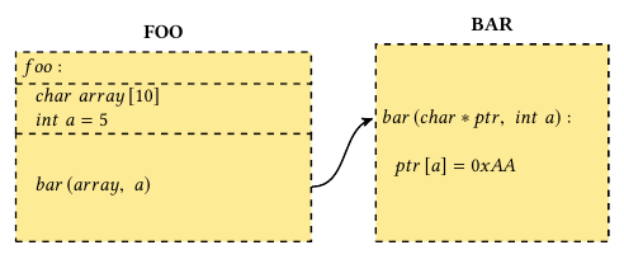
\includegraphics[width=\textwidth]{figures/cubicle_example_original.png}
         \caption{Original code of application FOO calling library BAR}
         \label{cubicleOriginal}
     \end{subfigure}
     \hfill
     \begin{subfigure}[b]{0.45\textwidth}
         %\centering
         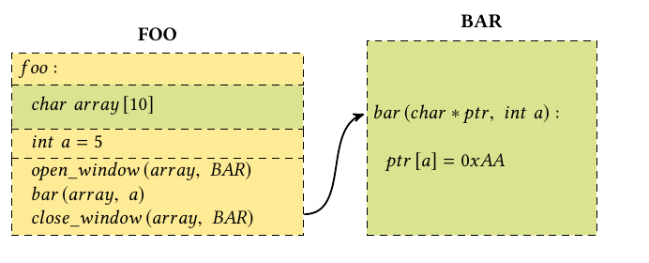
\includegraphics[width=\textwidth]{figures/cubicle_example_windows.png}
         \caption{Annotated code using Cubicles \textit{windows} to share memory after compilation}
         \label{cubicleWindow}
     \end{subfigure}
    \caption{To use Cubicle the developer basically needs to surround calls to other components, in this case BAR with \textit{windows}. Cubicle will derive isolated components and their (legitimate) interaction}
    \label{fig:CubicleAPI}
    \end{figure}

FlexOS~\cite{lefeuvre2021flexos} 
\begin{itemize}
    \item FlexOS is build on the ideas of library operating systems, in particular on the idea that 'everything is a library'. 
    \item This includes (micro)kernel components the system uses. 
    \item It is based on the Unikraft~\cite{kuenzer2021unikraft} library OS.
    \item FlexOS consists of a toolchain, a set of adapted libraries for all kinds of system/kernel functions (boot, networking, device drivers, memory access) and applications (e.g. nginx, redis, sqlite ...) and a set of supported 'Isolation Backends'. 
    \item Users provide the code for their application and a configuration specifying the libraries and backend to use and FlexOs will produce a custom, single-address space, single purpose OS for the compiled appliance.
    \item We do two things at the same time i) We isolate parts of the code from each other by extracting independent process steps from the composition code (build a DFG) and ii) We introduce backend specific communication mechanisms among the separated components. 
    \item FlexOS does only of this. 
    \item In particular, in the adapted libraries shared memory constructs as well as calls among different compartments (libraries) are marked with FlexOS specific placeholders. In the compilation process, the FlexOS toolchain replaces those placeholders with appropriate primitives for the selected 'Isolation Backend'. 
    \item \todo[inline]{At least the mechanism of keeping function calls abstract and making them concrete during compilation corresponds to the concrete implementation of channels in the backend. TODO: How exactly is shared state translated?}
\end{itemize}

\section{Compiling stateful imperative to Data Flow}
"Making State Explicit for Imperative Big Data Processing
"~\cite{fernandez2014making}:
\begin{itemize}
    \item identified problem: support arbitrary (Java) state in BigData (with high scalability) and recover state upon failure
    \item approach: infer dataflow and 'types of state access' to derive a 'stateful dataflow graph'(SDG)
    \item they explicitly focus on 'large states', where distribution of such state to several nodes is desirable both for performance/(storage/compute) capacity and for recovery after failure 
    \item SGD: "cyclic graph of pipelined data-parallel tasks, which exe-
cute on different nodes and access local in-memory state" \means no explicit scheduling
\item to identify 'partial' and 'partitioned' stateful objects, they require annotations from the programmer
\end{itemize}

"DFGenTool: A Dataflow Graph Generation Tool for Coarse Grain Reconfigurable Architectures "~\cite{mukherjee2017dfgentool}
\begin{itemize}
    \item based on LLVMIR
\end{itemize}


%\chapter{Conclusion}
\label{Chapter:Discussion}
%Isolating components of a kernel or larger programs from each other makes sense both for security reasons and for better scalability. But adapting existing code bases is time-consuming and complicates development and testing. This is also true, for example, when programs written for monolithic or unikernels have to be rewritten for microkernel-based systems like \md with isolated drivers and system components. The Ohua compiler tries to solve this problem by automatically identifying independent sections of a program and making them separate threads or processes, depending on the architecture chosen.\\

In this work we have looked at whether it is possible to compile programs with Ohua whose structure does not yet contain the desired independent components. Using the concrete example of a server application, we looked at which transformations are necessary to create a program in which the TCP/IP stack, the network interface and the user application are independent, stateful components. By means of a backend integration for the microkernel-based operating system \md, a program transformed in this way could be compiled directly from running on a uni- or monolithic kernel to running on a microkernel based OS. \\

To achieve this, the components must only be used once in the compiled program. The communication between them must be realized via the arguments of a single function call, and the control flow of the entire program must be adapted accordingly. As it turned out, part of this problem can be formally described by transformation to Continuation Passing Style and Defunctionalization, and could be further developed to transformations in Ohua. Other necessary steps are not possible without additional demands on the programmer. This includes, among other things, the identification of the target components if this is not apparent from the initial code structure. In general, lifting code into scope that was encapsulated in function or method calls is problematic because it is the programmer's responsibility to respect the constraints of the programming model, e.g. that function arguments need to be serializable for the selected backend. As the transformations that Ohua performs on the code become more complex, it may become more difficult for the programmer to know in which areas of the code to adhere to the programming model. \\

Comparing Ohua with other approaches for compartmentalization we have seen that Ohua is more flexible since it is not directly build upon a single input language, compiler toolchain or particular hardware mechanism. However, as we have seen in the adaption to \md, we face the same problems when it comes to adaptations between different operating systems, namely that system calls can not be automatically identified from the syntax and replaced by Ohua. It might be worthwhile to consider adding annotations to Ohuas API in future versions, to enable e.g. the automatic encapsulation of components or the use of different data transfer mechanisms. Otherwise the input program already needs to use appropriate system calls and components, which contradicts the original idea of being able to develop the code independently of the target architecture. \\

For further work, we therefore need to clearly distinguish which transformations we can and want to implement in Ohua, and which steps should be left to the programmer.  



\appendix
\chapter{Appendix}
\label{Appendix}
\section{Odds and Ends}
\end{thesisdocument}
\end{document}